\documentclass[12pt]{article}

\usepackage{multirow}
\usepackage{amsmath}
\usepackage{amsfonts}
\usepackage{float}
\usepackage{fancyhdr}
\usepackage{graphicx}
\usepackage{setspace}
\usepackage[colorlinks=true,linkcolor=blue, citecolor=red]{hyperref}
\usepackage{url}
\usepackage[top=.75in, left=.75in, right=.75in, bottom=1in]{geometry}
\usepackage[utf8]{vietnam}

% For algorithm
\usepackage{mathtools}
\usepackage{algorithm}
 \usepackage[noend]{algpseudocode}
 \usepackage{setspace, etoolbox, caption}

\usepackage{algpseudocode}


% ============ CODE ============
\usepackage{listingsutf8}%\usepackage{listings}
\usepackage{xcolor}
\definecolor{codegreen}{rgb}{0,0.6,0}
\definecolor{codegray}{rgb}{0.5,0.5,0.5}
\definecolor{codepurple}{rgb}{0.58,0,0.82}
\definecolor{backcolour}{rgb}{0.95,0.95,0.92}

% Styling for the code.
\lstdefinestyle{mystyle}{
    backgroundcolor=\color{backcolour},   
    commentstyle=\color{codegreen},
    keywordstyle=\color{magenta},
    numberstyle=\tiny\color{codegray},
    stringstyle=\color{codepurple},
    basicstyle=\ttfamily\footnotesize,
    breakatwhitespace=false,         
    breaklines=true,                 
    captionpos=b,                    
    keepspaces=true,                 
    numbers=left,                    
    numbersep=5pt,                  
    showspaces=false,                
    showstringspaces=false,
    showtabs=false,                  
    tabsize=2
}
\lstset{style=mystyle}

% Disable indentation on new paragraphs
%\setlength{\parindent}{0pt}

% Line spacing 1.5
\renewcommand{\baselinestretch}{1}

% Optional: graphic path
% \graphicspath{PATH_TO_GRAPHIC_FOLDER}

% To use Times font family, uncomment this row
% \usepackage{mathptmx}

% To use roman section / subsection, uncomment these rows
% \renewcommand{\thesection}{\Roman{section}}
% \renewcommand{\thesubsection}{\thesection.\Roman{subsection}}

% Define course name, report name and report title.
\newcommand{\coursename}{Thực hành - Lập trình cho Trí tuệ Nhân tạo}
\newcommand{\reportname}{Trò chơi Mê cung}
\newcommand{\reporttitle}{Báo cáo Đồ án}

\newcommand{\studentname}{Đinh Đức Anh Khoa (23122001)\\Nguyễn Đình Hà Dương (23122002)\\Nguyễn Lê Hoàng Trung (23122004)\\Đinh Đức Tài (23122013)}
\newcommand{\teachername}{Th.S Nguyễn Trần Duy Minh}

\newcommand{\leftfooter}{\LaTeX\ by \href{https://github.com/ductai05}{Duc Tai Dinh}}

% ============ HEADER AND FOOTER ============
% Header length
\setlength{\headheight}{29.43912pt}

% Footer page number would be on the lower-right corner
\pagestyle{fancy}
\fancyfoot{}
\fancyfoot[R]{Trang \thepage}

\lhead{\reporttitle}
\rhead{
Trường Đại học Khoa học Tự nhiên - ĐHQG HCM\\
\coursename
}
\lfoot{\leftfooter}

% ============ DOCUMENT ============
\begin{document}
\begin{titlepage}
\newcommand{\HRule}{\rule{\linewidth}{0.5mm}}
\centering

\textsc{\LARGE đại học quốc gia tphcm}\\[1.5cm]
\textsc{\Large trường đại học khoa học tự nhiên}\\[0.5cm]
\textsc{\large khoa công nghệ thông tin}\\[0.5cm]
\textsc{lớp trí tuệ nhân tạo khóa 2023 - 23TNT1}\\[0.5cm]

\HRule \\[0.4cm]
{ 
\huge{\bfseries{\reporttitle}}\\[0.5cm]
\large{\bfseries{Đề tài: \reportname}}
}\\[0.4cm]
\HRule \\[0.5cm]

\textbf{\large Môn học: \coursename}\\[0.5cm]

\begin{minipage}[t]{0.5\textwidth}
\begin{flushleft} \large
\emph{Sinh viên thực hiện:}\\
\studentname
\end{flushleft}
\end{minipage}
~
\begin{minipage}[t]{0.4\textwidth}
\begin{flushright} \large
\emph{Giáo viên hướng dẫn:} \\
\teachername
\end{flushright}
\end{minipage}\\[2cm]

{\large \today}\\[1cm]


\includegraphics[scale=.25]{img/hcmus-logo.png}\\[1cm] 

\vfill
\end{titlepage}
	
	
\tableofcontents
\pagebreak

\section{Giới thiệu}

\paragraph{}{\textbf{Đây là bài báo cáo cho Đồ án Trò chơi Mê cung, môn Thực hành - Lập trình cho Trí tuệ Nhân tạo, lớp 23TNT1, Khoa Công nghệ thông tin, Trường Đại học Khoa học tự nhiên - Đại học Quốc gia TP.HCM.}}

\paragraph{}{\textbf{Đồ án được thực hiện bởi nhóm các thành viên:}}

\begin{itemize}
    \item Đinh Đức Anh Khoa (23122001)
    \item Nguyễn Đình Hà Dương (23122002)
    \item Nguyễn Lê Hoàng Trung (23122004)
    \item Đinh Đức Tài (23122013)
\end{itemize}

\section{Phân công nhiệm vụ, đánh giá mức độ hoàn thành}

\textbf{Bảng phân công nhiệm vụ cho từng thành viên:}

\begin{table}[H]
\centering
\begin{tabular}{|c|c|l|c|}
\hline
\textbf{Họ và tên} & \textbf{MSSV} & \multicolumn{1}{c|}{\textbf{Nhiệm vụ}} & \textbf{\begin{tabular}[c]{@{}c@{}}Mức độ\\ hoàn thành\end{tabular}} \\ \hline
\begin{tabular}[c]{@{}c@{}}Đinh Đức \\ Anh Khoa\end{tabular} & 23122001 & \begin{tabular}[c]{@{}l@{}}- Viết báo cáo thuật toán: A*, BFS, so sánh A* và BFS,\\ phát sinh mê cung, hệ thống gợi ý đường đi\\ - Viết code thuật toán A*\\ - Game tester, quay demo\end{tabular} & Tốt (100\%) \\ \hline
\begin{tabular}[c]{@{}c@{}}Nguyễn Đình\\ Hà Dương\end{tabular} & 23122002 & \begin{tabular}[c]{@{}l@{}}- Design hình ảnh menu và game\\ - Viết code giao diện menu, gameplay; xử lý đồ hoạ và xử\\ lý trong gameplay\end{tabular} & Tốt (100\%) \\ \hline
\begin{tabular}[c]{@{}c@{}}Nguyễn Lê\\ Hoàng Trung\end{tabular} & 23122004 & \begin{tabular}[c]{@{}l@{}}- Viết code và báo cáo thuật toán BFS\\ - Viết code giao diện gameplay; xử lí đồ hoạ, dữ liệu của \\ ma trận và xử lí thao tác, chuyển động của nhân vật\end{tabular} & Tốt (100\%) \\ \hline
\begin{tabular}[c]{@{}c@{}}Đinh \\ Đức Tài\end{tabular} & 23122013 & \begin{tabular}[c]{@{}l@{}}- Viết báo cáo. Viết thuật toán mê cung sinh năng lượng.\\ - Viết code giao diện, chức năng menu; code database\\ - Thiết kế cấu trúc phần mềm\end{tabular} & Tốt (100\%) \\ \hline
\end{tabular}
\end{table}

\newpage
\textbf{Tự đánh giá mức độ hoàn thành của từng yêu cầu:}

% Please add the following required packages to your document preamble:
% \usepackage{multirow}
\begin{table}[H]
\centering
\begin{tabular}{|cc|l|c|}
\hline
\multicolumn{2}{|c|}{\textbf{\begin{tabular}[c]{@{}c@{}}Các yêu \\ cầu chính\end{tabular}}} & \multicolumn{1}{c|}{\textbf{Nội dung}} & \textbf{\begin{tabular}[c]{@{}c@{}}Tự đánh giá mức \\ độ hoàn thành\end{tabular}} \\ \hline
\multicolumn{1}{|c|}{\multirow{2}{*}{\begin{tabular}[c]{@{}c@{}}Xử lí\\ tài\\ khoản\end{tabular}}} & \begin{tabular}[c]{@{}c@{}}Đăng \\ nhập\end{tabular} & \begin{tabular}[c]{@{}l@{}}Người dùng nhập tên đăng nhập và mật khẩu để đăng \\ nhập vào game\end{tabular} & Tốt (100\%) \\ \cline{2-4} 
\multicolumn{1}{|c|}{} & \begin{tabular}[c]{@{}c@{}}Đăng \\ kí\end{tabular} & \begin{tabular}[c]{@{}l@{}}Nếu người dùng chưa có tài khoản, phải điền tên và \\ mật khẩu để sử dụng\end{tabular} & Tốt (100\%) \\ \hline
\multicolumn{1}{|c|}{} & \begin{tabular}[c]{@{}c@{}}Chế \\ độ \\ chơi\end{tabular} & \begin{tabular}[c]{@{}l@{}}Lựa chọn chế độ chơi (tự chơi, tự động), độ khó \\ (dễ, trung bình, khó), phát sinh bản đồ (ngẫu nhiên, \\ tự chọn)\end{tabular} & Tốt (100\%) \\ \cline{2-4} 
\multicolumn{1}{|c|}{Menu} & \begin{tabular}[c]{@{}c@{}}Bảng \\ xếp\\ hạng\end{tabular} & \begin{tabular}[c]{@{}l@{}}Sau khi qua mỗi mê cung, người dùng sẽ được lưu \\ thời gian qua màn, số bước đã sử dụng từ đó lưu vào\\ bảng xếp hạng. Bảng xếp hạng được chia theo độ khó.\end{tabular} & Tốt (100\%) \\ \cline{2-4} 
\multicolumn{1}{|c|}{} & \begin{tabular}[c]{@{}c@{}}Thoát \\ game\end{tabular} & Kết thúc trò chơi & Tốt (100\%) \\ \hline
\multicolumn{2}{|c|}{\begin{tabular}[c]{@{}c@{}}Lưu \\ trạng thái \\ người chơi\end{tabular}} & \begin{tabular}[c]{@{}l@{}}Ở chế độ tự chơi, khi người chơi chưa hoàn thành\\ nhưng đã nghỉ giữa chừng thì phải lưu lại được \\ trạng thái và có thể load lại map được khi người \\ dùng quay lại chơi.\end{tabular} & Tốt (100\%) \\ \hline
\multicolumn{2}{|c|}{\textbf{\begin{tabular}[c]{@{}c@{}}Các yêu \\ cầu khác\end{tabular}}} & \multicolumn{1}{c|}{\textbf{Nội dung}} & \textbf{\begin{tabular}[c]{@{}c@{}}Tự đánh giá mức \\ độ hoàn thành\end{tabular}} \\ \hline
\multicolumn{2}{|c|}{\begin{tabular}[c]{@{}c@{}}Gợi ý \\ đường đi\end{tabular}} & \begin{tabular}[c]{@{}l@{}}Ở chế độ tự chơi, khi người dùng nhấn vào nút gợi \\ ý,  hệ thống sẽ hiển thị đường đi từ vị trí hiện tại \\ của nhân vật đến đích.\end{tabular} & Tốt (100\%) \\ \hline
\multicolumn{2}{|c|}{\begin{tabular}[c]{@{}c@{}}Âm nhạc, \\ hình nền\end{tabular}} & Tạo âm nhạc và hình nền cho trò chơi & Tốt (100\%) \\ \hline
\multicolumn{2}{|c|}{\begin{tabular}[c]{@{}c@{}}Lý thuyết \\ trò chơi\end{tabular}} & \begin{tabular}[c]{@{}l@{}}Cho trước số bước đi tối đa của Tâm là H, và phát \\ sinh ngẫu nhiên K viên năng lượng trong bản đồ.\\ Tìm đường đi ngắn nhất đến nhà Gia Huy, biết rằng \\ cứ mỗi bước đi sẽ mất 1 năng lượng và ăn được 1 \\ viên năng lượng sẽ có thêm $V_k$ năng lượng với\\ $V_k$ là giá trị phát sinh ngẫu nhiên thuộc \\ \{1, 2, 3, 4, 5\}. Giá trị của H và K cũng sẽ tương \\ ứng với các mức độ trò chơi.\end{tabular} & Khá (65\%) \\ \hline
\end{tabular}
\end{table}
\newpage
\section{Các thư viện và công nghệ}
\subsection{Python}
\paragraph{Ngôn ngữ lập trình Python} \cite{python}
\paragraph{}{Python là một ngôn ngữ lập trình thông dịch, hướng đối tượng, cấp cao với ngữ nghĩa động. Các cấu trúc dữ liệu tích hợp cấp cao của nó, kết hợp với kiểu động và liên kết động, làm cho Python rất hấp dẫn để phát triển ứng dụng nhanh, cũng như sử dụng như một ngôn ngữ kịch bản hoặc ngôn ngữ kết nối để kết nối các thành phần hiện có với nhau. Cú pháp đơn giản, dễ học của Python nhấn mạnh tính dễ đọc và do đó giảm chi phí bảo trì chương trình. Python hỗ trợ các mô-đun và gói, khuyến khích tính mô-đun của chương trình và tái sử dụng mã nguồn. Trình thông dịch Python và thư viện chuẩn phong phú có sẵn dưới dạng mã nguồn hoặc dạng nhị phân mà không mất phí cho tất cả các nền tảng chính, và có thể được phân phối tự do.}

\paragraph{Phiên bản}
\paragraph{}{Đồ án sử dụng Python phiên bản \textbf{3.11.9}.}

\subsection{Pygame}

\paragraph{Thư viện Pygame} \cite{pygame}
\paragraph{}{Pygame là một bộ mô-đun Python đa nền tảng được thiết kế để viết trò chơi điện tử. Pygame bao gồm đồ họa máy tính và thư viện âm thanh được thiết kế để sử dụng với ngôn ngữ lập trình Python.}

\paragraph{Phiên bản}
\paragraph{}{Đồ án sử dụng Pygame phiên bản \textbf{2.5.2}.}

\subsection{Pygame-menu} 

\paragraph{Thư viện Pygame-menu} \cite{pygame-menu}
\paragraph{}{Pygame-menu là một thư viện python-pygame để tạo menu và giao diện người dùng đồ họa (GUI). Pygame-menu hỗ trợ nhiều widget khác nhau, chẳng hạn như nút bấm, bộ chọn màu, đồng hồ, bộ chọn thả xuống, khung, hình ảnh, nhãn, bộ chọn, bảng, đầu vào văn bản, công tắc màu và nhiều hơn nữa, với nhiều tùy chọn để tùy chỉnh.}

\paragraph{Phiên bản}
\paragraph{}{Đồ án sử dụng Pygame-menu phiên bản \textbf{4.4.3}.}

\newpage
\section{Các thành phần trong code}
\subsection{Tổng quan về code}

\paragraph{Cấu trúc}
\paragraph{}{Các thành phần trong game được tổ chức như hình bên dưới:}
\begin{figure}[H]
    \centering
    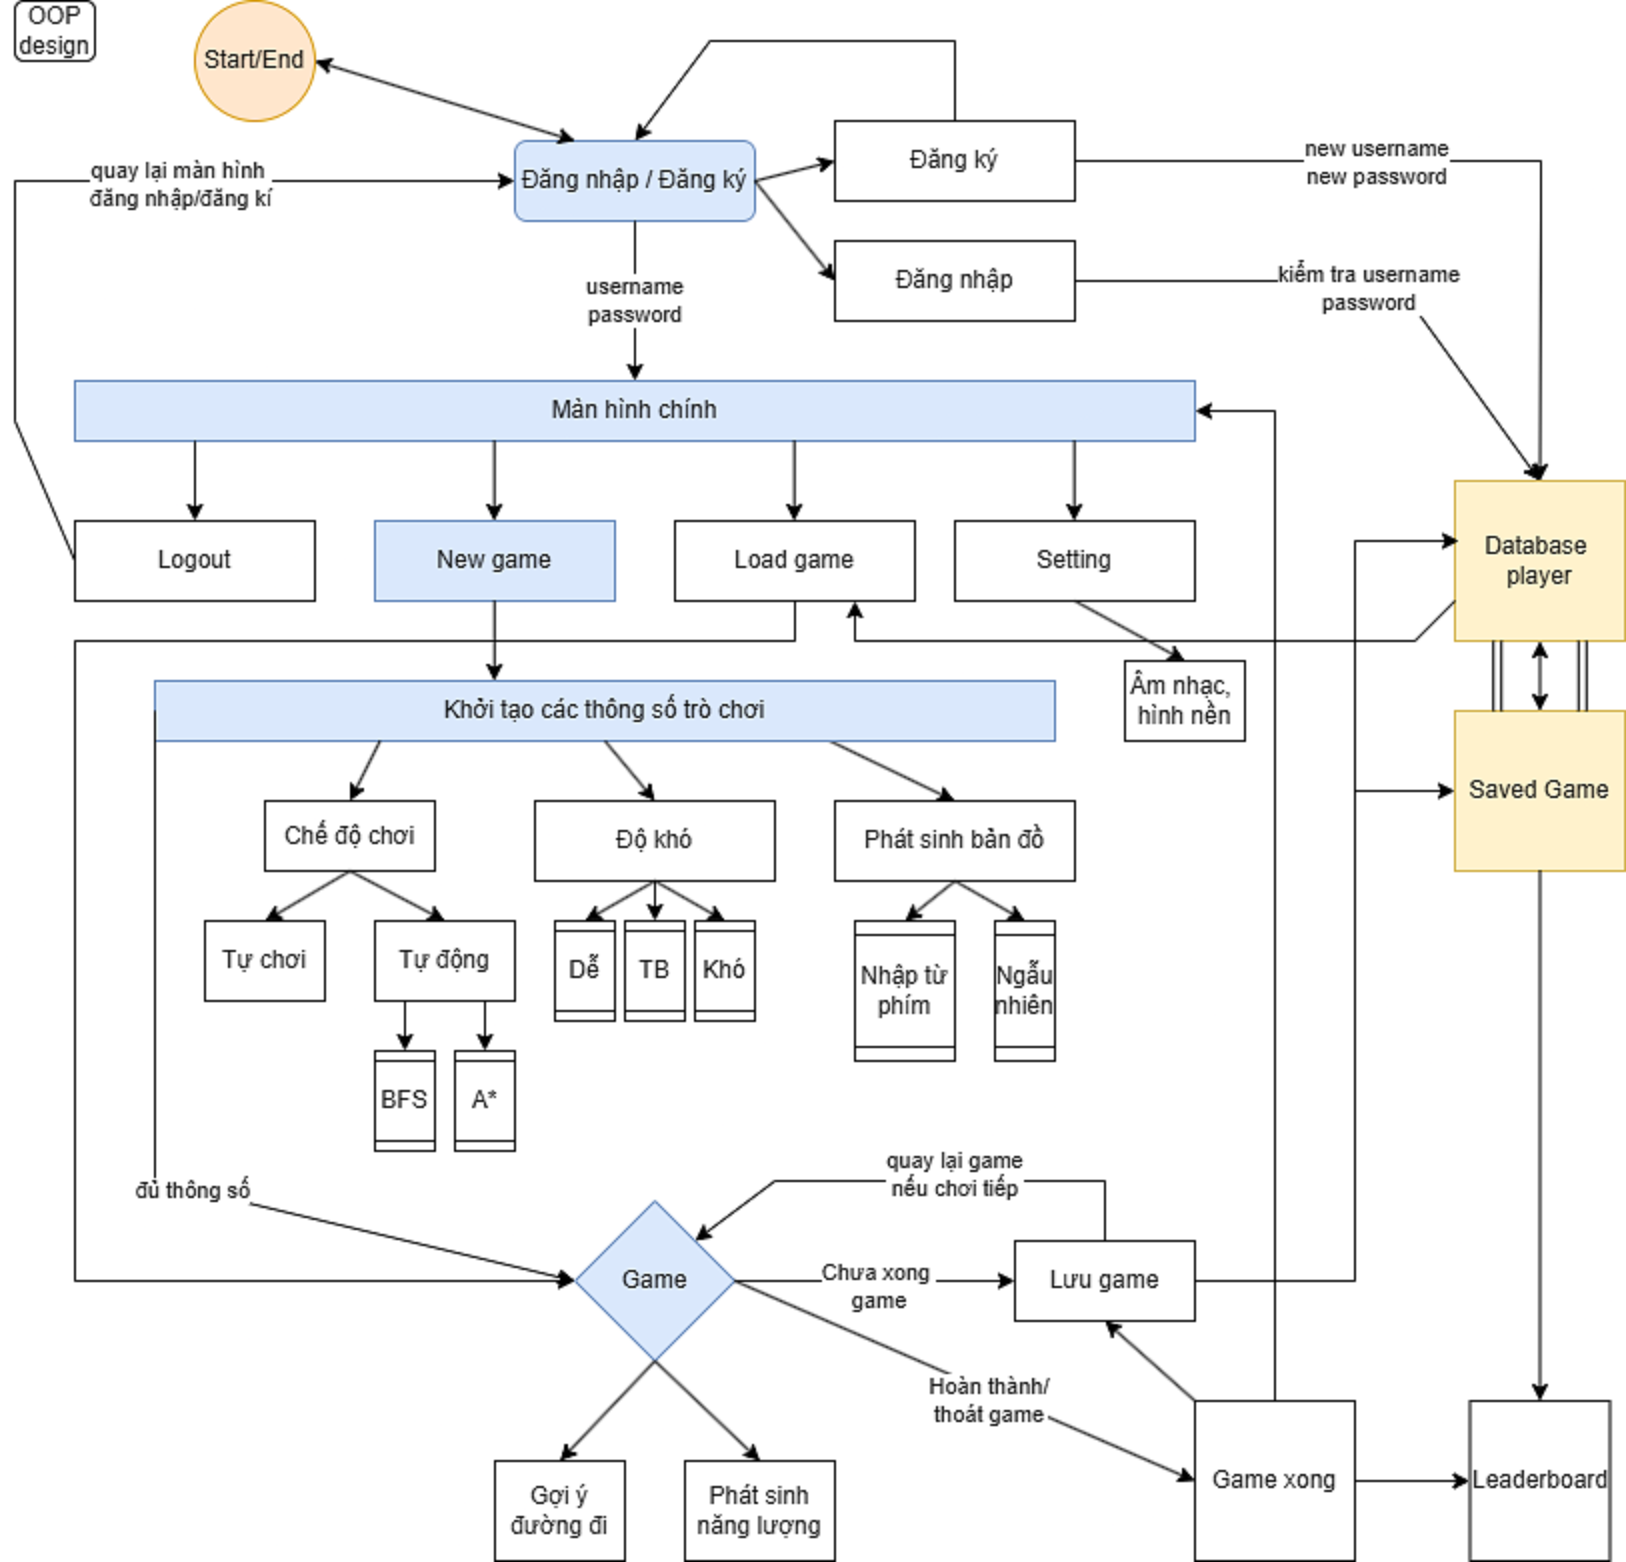
\includegraphics[width=1\linewidth]{img/pj_code.png}
    \caption{Sơ đồ tổ chức code}
    \label{fig:pj_code}
\end{figure}
\newpage

\paragraph{Phương pháp lập trình}
\paragraph{}{Code trong đồ án được tổ chức theo phương pháp lập trình hướng đối tượng. Điều này giúp code rõ ràng, rành mạch, không bị chồng chéo các biến và chức năng với nhau.}

\paragraph{Tổ chức code}
\paragraph{}{Code được tổ chức thành các file với đuôi $.py$. Mỗi file chứa các class, chịu trách nhiệm cho các chức năng riêng, trong đó:}
\begin{itemize}
    \item \textbf{main.py} : Gọi các tệp tin và class khác, khởi tạo trò chơi.

    \item \textbf{database.py} : Lưu trữ thông tin người dùng, các ván chơi và xử lí xuất nhập thông tin, gồm 1 class: \texttt{UserDatabase}

    \item \textbf{login\_startgame.py} : Xử lí giao diện đăng kí, đăng nhập, menu, gồm 2 class: \texttt{LoginMenu}, \texttt{MenuGame}

    \item \textbf{maze\_generator.py} : Khởi tạo các thuộc tính cho mê cung, gồm 2 class: \texttt{Cell}, \texttt{Maze}

    \item \textbf{maze\_solver.py} : Tìm đường đi cho mê cung, gồm 2 class: \texttt{priority\_queue}, \texttt{mazeSolver}

    \item \textbf{utils.py} : Xử lí thông tin của 1 thư mục, gồm 1 hàm \texttt{import\_folder}

    \item \textbf{tile.py} : Hiển thị hình ảnh lên một ô / màn hình (đường đi, gợi ý, đường thuật toán tìm kiếm...), gồm 3 class: \texttt{Goal}, \texttt{Hint}, \texttt{Auto}.

    \item \textbf{Display.py} : Tạo các nút bấm, đồng hồ, hộp văn bản, gồm 5 class: \texttt{Clock}, \texttt{Button}, \texttt{Button\_Image}, \texttt{TextBox}, \texttt{Display},

    \item \textbf{player.py} : Quản lí trạng thái và hành vi của nhân vật người chơi, gồm 1 class: \texttt{Player}
    
    \item \textbf{level.py} : Quản lí các thành phần của trò chơi, gồm 1 class: \texttt{Level}

    \item \textbf{game.py} : Khởi tạo 1 game, gồm 1 class: \texttt{Game}
    
\end{itemize}

\paragraph{Các file phương tiện khác}
\paragraph{}{Các file còn lại có mục đích hiển thị hình ảnh, âm thanh, font chữ,... được chia vào 4 thư mục:}

\begin{itemize}
    \item \textbf{assets} : Ảnh nền, hoạt hoạ game mặc định
    \item \textbf{Themebeach} : Ảnh nền với theme biển
    \item \textbf{font} : Các font chữ
    \item \textbf{sound} : Các file âm thanh
\end{itemize}
    

\subsection{Chi tiết các thành phần code}

\subsubsection{Vận hành database}

\paragraph{File database.py - class \texttt{UserDatabase}}

\begin{itemize}
    \item \textbf{Mục đích}: Xử lí các yêu cầu liên quan đến lưu trữ và trích xuất dữ liệu người dùng, các ván chơi, cài đặt mặc định...
    \item \textbf{Thuộc tính}:
    
    \begin{itemize}
        \item $filename$: tên file json - file lưu trữ thông tin.
        \item $users$: chứa thông tin của người dùng.
    \end{itemize}
    
    \item \textbf{Phương thức}:

    \begin{itemize}
        \item $load\_data$: Tải dữ liệu từ file json vào thuộc tính $users$.
        \item $save\_data$: Lưu dữ liệu của thuộc tính $users$ vào file json.
        \item $register\_user$: Đăng kí một người dùng mới, lưu vào file json.
        \item $login\_user$: Kiểm tra tính hợp lệ của username và password với dữ liệu hiện có.
        \item $load\_users$: Trả về toàn bộ dữ liệu của một người chơi.
        \item $load\_game$: Trả về dữ liệu của một game của một người chơi nào đó.
        \item $save\_game$: Lưu dữ liệu một game của một người chơi.
        \item $leaderboard$: Sắp xếp thứ hạng game của các người chơi, trả về thứ hạng theo độ khó.
    \end{itemize}
    
\end{itemize}

\subsubsection{Giao diện các menu}

\paragraph{File login\_startgame.py - class \texttt{LoginMenu}}

\begin{itemize}
    \item \textbf{Mục đích}: Tạo menu xử lí đăng nhập, đăng kí tài khoản người chơi.
    \item \textbf{Thuộc tính}:
    
    \begin{itemize}
        \item $surface$: Màn hình để hiển thị menu. Đây là một thuộc tính được khởi tạo dựa trên thư viện pygame-menu.
        \item $main\_menu$: Menu chính của phần đăng nhập, đăng kí. Đây là một thuộc tính được khởi tạo dựa trên thư viện pygame-menu.
        \item Ngoài ra còn có các thuộc tính như các menu con, button, widget, âm thanh... là thành phần cấu tạo nên $main\_menu$.
    \end{itemize}
    
    \item \textbf{Phương thức}:

    \begin{itemize}
        \item $check\_login$, $check\_register$: Kiểm tra tính hợp lệ của username và password được đăng nhập hoặc đăng kí, đưa ra thông báo.
        \item $reset\_noti\_login$, $reset\_noti\_regis$: Tạo thông báo lúc đăng kí/đăng nhập cho người chơi biết.
        \item $init\_theme$: Khởi tạo các cài đặt, hình ảnh, định dạng menu.
        \item $init\_login\_menu$, $init\_register\_menu$, $init\_main\_menu$, $init\_menu$: Khởi tạo menu và các thành phần của menu (dựa trên thư viện pygame-menu).
        \item $start$: Hàm dùng để gọi việc hiển thị menu đăng nhập, đăng kí.
    \end{itemize}
    
\end{itemize}

\paragraph{File login\_startgame.py - class \texttt{MenuGame}}

\begin{itemize}
    \item \textbf{Mục đích}: Tạo menu, xử lí các hoạt động tương tác với hệ thống của người chơi đã đăng nhập (bắt đầu game mới, tải một game đã chơi, cài đặt game, đăng xuất,...).
    \item \textbf{Thuộc tính}:
    
    \begin{itemize}
        \item $username$, $password$: Username và password của người chơi.
        \item $surface$: Màn hình để hiển thị menu. Đây là một thuộc tính được khởi tạo dựa trên thư viện pygame-menu.
        \item $main\_menu$: Menu chính khi người chơi đã đăng nhập. Đây là một thuộc tính được khởi tạo dựa trên thư viện pygame-menu.
        \item Ngoài ra còn có các thuộc tính như các menu con, button, widget, âm thanh... là thành phần cấu tạo nên $main\_menu$.
    \end{itemize}
    
    \item \textbf{Phương thức}:

    \begin{itemize}
        \item $update\_menu\_sound\_switch$, $change\_bgm$, $change\_sfx$: Cài đặt âm thanh.
        \item $change\_theme$: Thay đổi theme.
        \item $reset\_all\_setting$: Thiết lập các cài đặt trở về mặc định.
        \item $return\_to\_login$: Đăng xuất tài khoản và quay trở về menu đăng nhập, đăng xuất.
        \item $get\_data\_leaderboard$: Gọi dữ liệu từ database, sắp xếp tạo leaderboard.
        \item $start\_a\_saved\_game$: Bắt đầu một game đã được lưu.
        \item $init\_theme$: Khởi tạo các cài đặt, hình ảnh định dạng menu.
        \item $init\_start\_game$, $init\_load\_game$, $init\_leaderboard$, $init\_setting$, $init\_main\_menu$, $init\_menu$: Khởi tạo menu và các thành phần của menu (dựa trên thư viện pygame-menu).
        \item $start$: Hàm dùng để gọi việc hiển thị menu chính khi người chơi đã đăng nhập.
    \end{itemize}
    
\end{itemize}

\subsubsection{Khởi tạo mê cung và tìm đường đi}

\paragraph{File maze\_generator.py - class \texttt{Cell}}

\begin{itemize}
    \item \textbf{Mục đích}: Định nghĩa các thuộc tính và phương thức cho một ô trong mê cung.
    
    \item \textbf{Thuộc tính}:
        \begin{itemize}
            \item $x$, $y$: Toạ độ của ô trong ma trận.
            \item $pos$: Toạ độ hiển thị của ô trong screen.
            \item $width$, $wall\_width$ : Chiều rộng của ô, độ rộng của tường
        \end{itemize}
        
    \item \textbf{Phương thức}:
        \begin{itemize}
            \item $draw$: Vẽ hình ảnh trong 1 ô.
            \item $render$: Vẽ tường bao quanh.
            \item $neighbor$: Trả về tọa độ của các ô kề cạnh không bị ngăn cách bởi tường.
        \end{itemize}
\end{itemize}

\paragraph{File maze\_generator.py - class \texttt{Maze}}

\begin{itemize}
    \item \textbf{Mục đích}: Định nghĩa các thuộc tính và phương thức cho mê cung.
    
    \item \textbf{Thuộc tính}:
        \begin{itemize}
            \item $size$: Kích thước của mê cung
            \item $startX$, $startY$, $endX$, $endY$: Tọa độ ô bắt đầu và tọa độ ô kết thúc
            \item $width$, $wall\_width$ : Chiều rộng của ô, độ rộng của tường
            \item $grid$: Ma trận của mê cung
            \item $trace$: Tọa độ của ô trước đó đã đi vào
            \item $hint$: Gợi ý ô tiếp theo hướng đến điểm kết thúc
        \end{itemize}
        
    \item \textbf{Phương thức}:
        \begin{itemize}
            \item $breakWall$: Phá tường theo hướng.
            \item $mazeGenerate$: Sinh một mê cung. 
            \item $render$: Hiển thị mê cung.
            \item $makeHint$: Tạo gợi ý đường đi bằng BFS cho toàn bộ ô trong mê cung.
            \item $hint$: Trả về đường đi gợi ý cho người chơi hướng đến điểm kết thúc đến khi gặp ngã ba.
        \end{itemize}
\end{itemize}

\paragraph{File maze\_solver.py - class \texttt{priority\_queue}}

\begin{itemize}
    \item \textbf{Mục đích}: Khởi tạo, định nghĩa hàng đợi ưu tiên (priority queue)
    
    \item \textbf{Thuộc tính}:
        \begin{itemize}
            \item $heap$: Một danh sách chứa các phần tử trong heap.
        \end{itemize}
        
    \item \textbf{Phương thức}:
        \begin{itemize}
            \item $push$: Sử dụng phương thức $heappush$ từ mô-đun \texttt{heapq} để thêm một phần tử vào trong $heap$ (đảm bảo $heap$ có phần tử nhỏ nhất luôn ở đầu danh sách).
            \item $pop$: Sử dụng phương thức $heappop$ từ mô-đun \texttt{heapq}, loại bỏ và trả về phần tử nhỏ nhất từ $heap$.
            \item $peek$: Trả về phần tử nhỏ nhất trong $heap$ mà không loại bỏ nó.
            \item $\_\_len\_\_$: Trả về số lượng phần tử hiện tại trong $heap$.
        \end{itemize}
\end{itemize}

\paragraph{File maze\_solver.py - class \texttt{MazeSolver}}

\begin{itemize}
    \item \textbf{Mục đích}: Sử dụng các thuật toán tìm đường (A*, BFS) để trả về đường đi.
    
    \item \textbf{Thuộc tính}:
        \begin{itemize}
            \item $maze$: Một mê cung, được khởi tạo dựa trên class $Maze$ (file maze\_generator.py)
        \end{itemize}
        
    \item \textbf{Phương thức}:
        \begin{itemize}
            \item $tracePath$: Trả về danh sách gồm thứ tự di chuyển (đường đi) tìm được, bao gồm cả điểm bắt đầu và kết thúc.
            \item $AStarSearch$: Chạy thuật toán A* và trả về danh sách thứ tự thăm các ô.
            \item $BFS$: Chạy thuật toán BFS và trả về danh sách thứ tự thăm các ô.
        \end{itemize}
\end{itemize}


\subsubsection{Xử lí game}

\paragraph{File utils.py - function \texttt{import\_folder}}
\begin{itemize}
    \item \textbf{Mục đích}: Nhập và xử lí hình ảnh từ một thư mục, trả về surface (pygame) đã được chỉnh sửa kích thước.
\end{itemize}

\paragraph{File tile.py - class \texttt{Goal}, \texttt{Hint}, \texttt{Auto}}
\begin{itemize}
    \item \textbf{Mục đích}: Hiển thị ảnh đường đi thuật toán tìm kiếm, đường đã đi, chiến thắng game.
    \item \textbf{Các class}:
    \begin{itemize}
        \item \texttt{Goal}: Vẽ thông báo chiến thắng.
        \item \texttt{Hint}: Vẽ đường đã đi qua.
        \item \texttt{Auto}: Vẽ thuật toán tìm kiếm.
    \end{itemize}
\end{itemize}

\paragraph{File Display.py - class \texttt{Clock}, \texttt{Button}, \texttt{Button\_Image}, \texttt{TextBox}, \texttt{Display}}
\begin{itemize}
    \item \textbf{Mục đích}: Tạo giao diện người dùng với các nút bấm, đồng hồ, hộp văn bản.
    \item \textbf{Các class}:
    \begin{itemize}
        \item \texttt{Clock}: Quản lý thời gian, gồm phút, giây và có các phương thức để cập nhật và hiển thị thời gian.
        \item \texttt{Button}: Quản lý nút bấm đơn giản với các khả năng tương tác với nút bấm đó.
        \item \texttt{Button\_Image}: Quản lý một nút bấm với hình ảnh, bao gồm cả hình ảnh khi nhấn và âm thanh khi nhấn.
        \item \texttt{TextBox}: Quản lý một hộp văn bản.
        \item \texttt{Display}: Hiển thị các đối tượng \texttt{Clock}, \texttt{Button}, \texttt{Button\_Image}, \texttt{TextBox} lên màn hình.
    \end{itemize}
\end{itemize}


\paragraph{File level.py - class \texttt{Level}}
\begin{itemize}
    \item \textbf{Mục đích}: Quản lí trò chơi, bao gồm người chơi, các thành phần của mê cung, tìm kiếm đường đi, hiển thị gợi ý...
    \item \textbf{Thuộc tính}:
        \begin{itemize}
            \item $game$: Đối tượng Game, gồm các thông tin ban đầu của trò chơi.
            \item $player$: Đối tượng Player, quản lí hoạt ảnh nhân vật.
            \item $solver$: Đối tượng MazeSolver, tìm đường đi trong mê cung bằng thuật toán.
            \item Ngoài ra còn có các thuộc tính khác để xử lí trò chơi.
        \end{itemize}
    \item \textbf{Phương thức}:
        \begin{itemize}
            \item $pack\_data$: Trả về dữ liệu trạng thái của người chơi và các gợi ý để lưu hoặc truyền dữ liệu.
            \item $getAuto$: Tìm đường đi dựa trên thuật toán cho trước.
            \item $run$: Vẽ mê cung, hiệu ứng, gợi ý,..., xử lí logic game, điều kiện thắng.
        \end{itemize}
\end{itemize}

\paragraph{File player.py - class \texttt{Player}}
\begin{itemize}
    \item \textbf{Mục đích}: Quản lý trạng thái và hành vi của nhân vật người chơi trong trò chơi, bao gồm việc xử lý đồ họa, di chuyển, và tương tác với môi trường mê cung.
    \item \textbf{Thuộc tính}:
        \begin{itemize}
            \item $maze$, $level$: Mê cung, lớp level
            \item $tilesize$: Kích thước của mỗi ô trong lưới.
        \end{itemize}
    \item \textbf{Phương thức}:
        \begin{itemize}
            \item $import\_player\_assets$: Gọi dữ liệu hoạt ảnh nhân vật.
            \item $input$: Xử lí đầu vào từ người chơi.
            \item $move$: Xử lí nhân vật di chuyển.
            \item $getPosition$: Lấy vị trí hiện tại của người chơi.
            \item $animate$: Biểu diễn hình ảnh nhân vật.
            \item $getHint$: Lấy gợi ý đường đi.
            \item $update$: Cập nhật hình ảnh nhân vật.
        \end{itemize}
\end{itemize}

\paragraph{File game.py - class \texttt{Game}}
\begin{itemize}
    \item \textbf{Mục đích}: Khởi tạo một game.
    \item \textbf{Thuộc tính}:
        \begin{itemize}
            \item $mode\_play$: Chế độ chơi (Player, Auto (A*), Auto (BFS))
            \item $difficult$, $start$, $end$: Kích thước bản đồ, toạ độ bắt đầu, đích đến. 
            \item $username$, $game\_name$: Tên người chơi, tên của game đang chơi.
            \item $step$: Số bước người chơi đã đi.
            \item Ngoài ra còn có các thuộc tính khác được khởi tạo từ các file xử lí game.
        \end{itemize}
    \item \textbf{Phương thức}:
        \begin{itemize}
            \item $pack\_data$: Gom dữ liệu của game để đưa tới database.
            \item $run$: Bắt đầu chạy game.
        \end{itemize}
\end{itemize}
\newpage
\section{Thuật toán phát sinh mê cung, các thuật toán tìm đường và gợi ý đường đi}

%--------------------------
%      Randomized DFS
%--------------------------

\subsection{Thuật toán phát sinh mê cung: Randomized DFS} 

\paragraph{}{Trong chương trình, chúng tôi sử dụng thuật toán \textbf{duyệt theo chiều sâu ngẫu nhiên} (randomized DFS) \cite{randomizeddfs} để sinh ra một mê cung. Thuật toán này sẽ sinh ra một mê cung có dạng cây. Tức là nếu coi mỗi ô trong ma trận là một đỉnh của đồ thị thì đồ thị này sẽ liên thông và không có chu trình. Điều này giúp đảm bảo từ một ô, ta có thể đi đến bất kỳ ô nào khác trong mê cung bằng một con đường duy nhất.}

\paragraph{}{Ban đầu, mê cung là một ma trận gồm có các ô trống, mỗi ô trống sẽ có 4 bức tường bao xung quanh.}

\begin{figure}[H]
    \centering
    
\includegraphics[width=0.3\linewidth]{img/init-maze-1.png}
    \caption{Ma trận các ô trống}
    \label{fig:init-maze-1}
\end{figure}

\paragraph{Thuật toán}
\paragraph{}{Thuật toán bắt đầu từ một ô bất kỳ trong mê cung, sau đó được thực hiện theo các bước:}

\paragraph{}{\textbf{Bước 1:} Gọi ô hiện tại đang được duyệt là ô $(x, y)$, ta thực hiện đánh dấu ô này là đã được duyệt qua.}
\paragraph{}{\textbf{Bước 2:} Lần lượt chọn các ô xung quanh chung cạnh với ô $(x, y)$ theo một thứ tự ngẫu nhiên. Tạm gọi ô đang được chọn là ô $(nx, ny)$.}
\paragraph{}{\textbf{Bước 3:} Nếu ô $(nx, ny)$ chưa được duyệt thì ta gọi đệ quy duyệt tới ô đó và xóa đi bức tường giữa ô $(x, y)$ và ô $(nx, ny)$. Ngược lại không làm gì cả.}


\paragraph{}{Sau khi thực hiện xong thuật toán ta được một mê cung thỏa mãn tính chất ở trên.}

\begin{figure}[H]
    \centering
    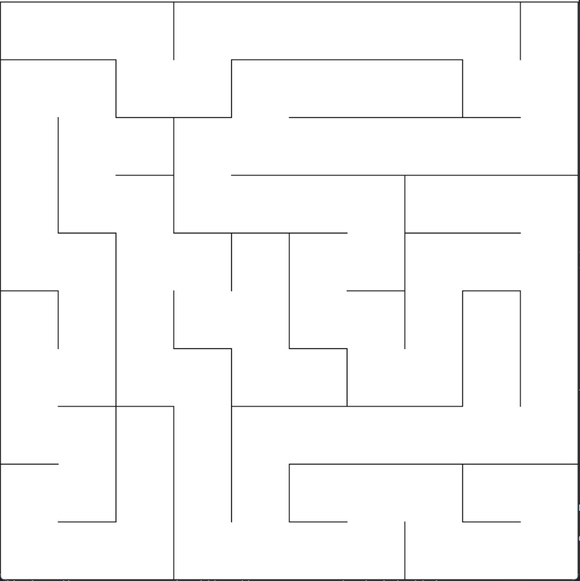
\includegraphics[width=0.3\linewidth]{img/init-maze-2.png}
    \caption{Mê cung được phát sinh sau khi thực hiện thuật toán}
    \label{fig:init-maze-2}
\end{figure}

\paragraph{Mã giả}{Thuật toán sinh mê cung randomized DFS}

\begin{algorithm}[H]
\caption{Randomized DFS}
\label{alg:rdfs}
\begin{algorithmic}
\Function {randomizedDFS}{\textit{x}, \textit{y}} 
\State // Đánh dấu đã duyệt ô (x, y)
\State $visited(x, y) \gets True$ 
\State
\State // Lấy danh sách các ô xung quanh (x, y) theo thứ tự ngẫu nhiên
\State $to\_visit \gets random\_shuffle(neighbor(x, y))$ 
\State

\For {$(nx, ny) \in to\_visit$}
\If {$visited(x, y) == False$}
\State loại bỏ bức tường nằm giữa hai ô (x, y) và (nx, ny)
\State randomizedDFS(nx, ny)
\EndIf
\EndFor
\EndFunction

\end{algorithmic}
\end{algorithm}

%--------------------------
%       BFS
%--------------------------

\subsection{Thuật toán tìm đường: BFS}
\paragraph{}{Thuật toán \textbf{duyệt đồ thị ưu tiên chiều rộng} \textit{(Breadth-first search - BFS)} là một trong những thuật toán tìm kiếm cơ bản và thiết yếu trên đồ thị. Ứng dụng của BFS có thể giúp ta giải quyết tốt một số bài toán trong thời gian và không gian \textbf{tối thiểu}. Đặc biệt là bài toán tìm kiếm đường đi ngắn nhất từ một đỉnh gốc tới tất cả các đỉnh khác. Trong bài toán tìm đường đi trong mê cung này, ta sẽ coi mỗi ô của mê cung là \textbf{1 đỉnh}, nếu từ 1 ô này có thể sang 1 ô khác thì sẽ có \textbf{1 cạnh} nối giữa 2 đỉnh này.}

\paragraph{Cơ chế hoạt động}
\paragraph{}{Từ một điểm xuất phát sẽ duyệt các điểm xung quanh có thể tới được, từ các điểm đã được duyệt đó sẽ thực hiện lại cơ chế trên để duyệt sang các điểm xung quanh khác, cứ như vậy cho đến khi duyệt tất cả các nhánh để tìm được nhánh có chứa đích đến thì dừng lại. Thứ tự ưu tiên của một đường đi thuật toán BFS là những đỉnh nào gần đỉnh xuất phát hơn sẽ được duyệt trước.}

\paragraph{Thuật toán}
\paragraph{}{Thuật toán sử dụng một hàng đợi (queue) để chứa các đỉnh. Các đỉnh này sau đó sẽ được duyệt theo quy tắc FIFO (first-in, first-out) của \textit{queue}. Tức là đỉnh nào vào \textit{queue} trước sẽ được duyệt trước.}

\paragraph{}{\textbf{Bước 1:} Khởi tạo}
\begin{itemize}
    \item Các đỉnh đều ở trạng thái chưa được đánh dấu, ngoại trừ đỉnh xuất phát \textbf{s} đã được đánh dấu.
    \item Một hàng đợi ban đầu chỉ chứa 1 phần tử là \textbf{s}.
\end{itemize}
\paragraph{}{\textbf{Bước 2:} Lặp lại các bước sau cho đến khi hàng đợi rỗng:}
\begin{itemize}
    \item Lấy đỉnh \textbf{u} ra khỏi hàng đợi.
    \item Xét tất cả những đỉnh \textbf{v} kề với \textbf{u} mà chưa được đánh dấu, với mỗi đỉnh \textbf{v} đó:
    \begin{itemize}
        \item Đánh dấu \textbf{v} đã thăm.
        \item Lưu lại vết đường đi từ \textbf{u} đến \textbf{v}.
        \item Đẩy \textbf{v} vào trong hàng đợi.
    \end{itemize}
\end{itemize}

\paragraph{Mã giả}{Thuật toán tìm đường BFS}

\begin{algorithm}[H]
\caption{BFS}
\label{alg:bfs}
\begin{algorithmic}
\Function {BFS}{\textit{startNode}, \textit{endNode}} // Đưa vào đỉnh bắt đầu và kết thúc

\State // Danh sách đỉnh cần duyệt sẽ được đưa vào một hàng đợi
\State $queue  \gets$ hàng\_đợi\_rỗng
\State đưa $startNode$ vào $queue$
\State
\State // Khởi tạo mảng 1 chiều visited đánh dấu những đỉnh đã thăm, giá trị khởi tạo là \textit{chưa thăm }
\State $visited[startNode] \gets$ đã thăm 
\State
\While{$queue$ không rỗng}
\State $currentNode \gets$ đỉnh tiếp theo trong queue
\If{$currentNode == endNode$}
\State \Return tồn tại đường đi từ đỉnh bắt đầu đến đỉnh kết thúc
\EndIf
\State Loại bỏ $currentNode$ khỏi $queue$
\For{$each neighbor \in$ các\_đỉnh\_kề$(currentNode)$} // duyệt các đỉnh kề đỉnh hiện tại
\If {$currentNode$ không thể tới được $neighbor$}
\State $continue$
\EndIf
\State $visited[neighbor] \gets$ đã thăm
\State đưa $neighbor$ vào $queue$
\EndFor

\Return không tồn tại đường đi từ đỉnh bắt đầu đến đỉnh kết thúc
\EndWhile
\EndFunction
\end{algorithmic}
\end{algorithm}

\paragraph{}{\textbf{Độ phức tạp thời gian:} Gọi $|V|$ là số lượng đỉnh và $|E|$ là số lượng cạnh của mê cung. Độ phức tạp thời gian của thuật toán này là $O(|V|+|E|)$.}

%--------------------------
%       A*
%--------------------------

\subsection{Thuật toán tìm đường: A*} 
\paragraph{}{A* \cite{astar} là giải thuật tìm kiếm trong đồ thị, tìm đường đi từ nút hiện tại đến đích sử dụng một hàm để ước lượng chi phí hay còn gọi là hàm heuristic. Từ trạng thái đường đi hiện tại, A* xây dựng tất cả các đường đi có thể, sử dụng hàm heuristic để đánh giá, tìm kiếm đường đi tối ưu và lưu giữ tập các lời giải trong một hàng đợi ưu tiên (priority queue). Thứ tự ưu tiên của một đường đi $x$ được quyết định bởi hàm $f(x) = g(x) + h(x)$.}
\paragraph{}{Trong đó:}
\begin{itemize}
    \item $g(x)$ là chi phí của đường đi từ nút xuất phát đến nút hiện tại.
    \item $h(x)$ là hàm đánh giá heuristic ước lượng chi phí từ nút hiện tại đến đích.
\end{itemize}
\paragraph{}{Hàm $f(x)$ có giá trị càng thấp thì độ ưu tiên càng cao. Có nghĩa là ta luôn ưu tiên duyệt các nút ở gần mục tiêu hơn. Nếu hàm heuristic $h$ có tính chất đơn điệu (hay nhất quán) tức thỏa mãn điều kiện $h(x) \leq d(x, y) + h(y)$ với mọi cạnh $x - y$ (ở đây $d(x, y)$ là độ dài cạnh $x - y$) thì thuật toán A* sẽ đảm bảo tìm ra một đường đi tối ưu.}
\paragraph{}{Vì bài toán tìm đường đi trong mê cung của ta là bài toán tìm đường đi trên cây có nghĩa là tồn tại một đường đi duy nhất từ đỉnh bắt đầu đến đỉnh kết thúc mà không đi qua một đỉnh quá hai lần nên ta không cần quan tâm đến tính đơn điệu của hàm heuristic. Điều này sẽ khiến thuật toán chạy nhanh hơn trong đa phần trường hợp. Trong chương trình, chúng tôi sử dụng hàm heuristic là bình phương khoảng cách euclid giữa điểm hiện tại và điểm kết thúc trong mê cung. Nói cách khác, nếu đỉnh hiện tại là ô $(x, y)$ và đỉnh kết thúc là ô $(endX, endY)$, ta có hàm heuristic:}

$$h(x, y) = (endX - x)^2 + (endY - y)^2$$

\paragraph{}{Khi di chuyển qua một ô thì độ dài đường đi tăng thêm 1 nên nếu đỉnh hiện tại là ô $(x, y)$ và đỉnh tiếp theo là ô $(u, v)$, ta có:}

$$g(u, v) = g(x, y) + 1$$
\paragraph{}{Vậy ta có \textbf{độ ưu tiên} cho ô $(u, v)$ nếu ô trước đó là ô $(x, y)$:
\begin{align*}
f(u, v) &= g(u, v) + h(u, v) \\
&= [g(x, y) + 1] + [(endX - u)^2 + (endY - v)^2]
\end{align*}}

\paragraph{}{\textbf{Mã giả} cho thuật toán A*:}


\begin{algorithm}[H]
\caption{A*}
\label{alg:rdfs}
\begin{algorithmic}
\Function {AStar}{\textit{startNode}, \textit{endNode}} // Đưa vào đỉnh bắt đầu và kết thúc
\State // Danh sách đỉnh cần duyệt sẽ được đưa vào một hàng đợi ưu tiên
\State $openSet \gets priority\_queue()$
\State // Chi phí của đường  từ điểm xuất phát đến điểm hiện tại
\State $g \gets$ \{giá trị các đỉnh: $\infty \forall$ đỉnh và 0 với đỉnh bắt đầu\}
\State // Tổng chi phí 
\State $f \gets$ \{giá trị các đỉnh: $\infty \forall$ đỉnh và $heuristic(startNode)$ với đỉnh bắt đầu\}
\State
\State Đưa cặp $startNode$ cùng chi phí $f(startNode)$ vào $openSet$
\While{$openSet$ không rỗng}
\State $currentNode \gets$ đỉnh trong openSet có tổng chi phí thấp nhất
\If{$currentNode == endNode$}
\State \Return tìm thấy đường đi
\EndIf
\State Loại bỏ $currentNode$ khỏi $openSet$
\State
\State // duyệt qua các đỉnh kề hợp lệ với đỉnh hiện tại
\For{$each$ $neighbor \in$ các\_đỉnh\_kề$(currentNode)$}
\State $newG \gets g(currentNode) + 1$
\State$ newF \gets newG + heuristic(currentNode)$
\If{$newG < g(neighbor)$}
\State $g(neighbor) \gets newG$
\State $f(neighbor) \gets newF$
\State đưa cặp $neighbor$ và $f(neighbor)$ vào $openSet$
\EndIf
\EndFor
\EndWhile
\Return thất bại, không tìm thấy đường đi
\EndFunction
\end{algorithmic}
\end{algorithm}

\paragraph{Độ phức tạp thời gian}
\paragraph{}{Độ phức tạp thời gian của thuật toán A* phụ thuộc vào đánh giá heuristic. Trong trường hợp tệ nhất, A* sẽ có độ phức tạp là $O(b^d)$ với $b$ là số cạnh trung bình của mỗi đỉnh và $d$ là số lượng nút trên đường đi tối ưu từ đỉnh bắt đầu đến đỉnh kết thúc. Mặc dù vậy, A* vẫn là một trong những thuật toán tìm kiếm đường đi tốt nhất trong hầu hết các trường hợp.}

\paragraph{Ví dụ minh hoạ}
\paragraph{}{Trong ví dụ này ta chỉ quan tâm đến cách thuật toán A* hoạt động trong một ma trận bất kỳ, không phải cách thuật toán hoạt động ở trong một mê cung. Giả sử ta có một ma trận kích thước $10 * 10$ như \hyperref[fig:astar_pic1]{hình 4} với ô màu đỏ là ô xuất phát và ô màu xanh là ô kết thúc. Các viền màu đen đậm hơn bên ngoài và viền màu đỏ ở trong là các bức tường. Ở đây, ta sẽ lập sẵn các bảng giá trị cho từng hàm để mô tả thuật toán tốt hơn.}

\begin{figure}[H]
    \centering
    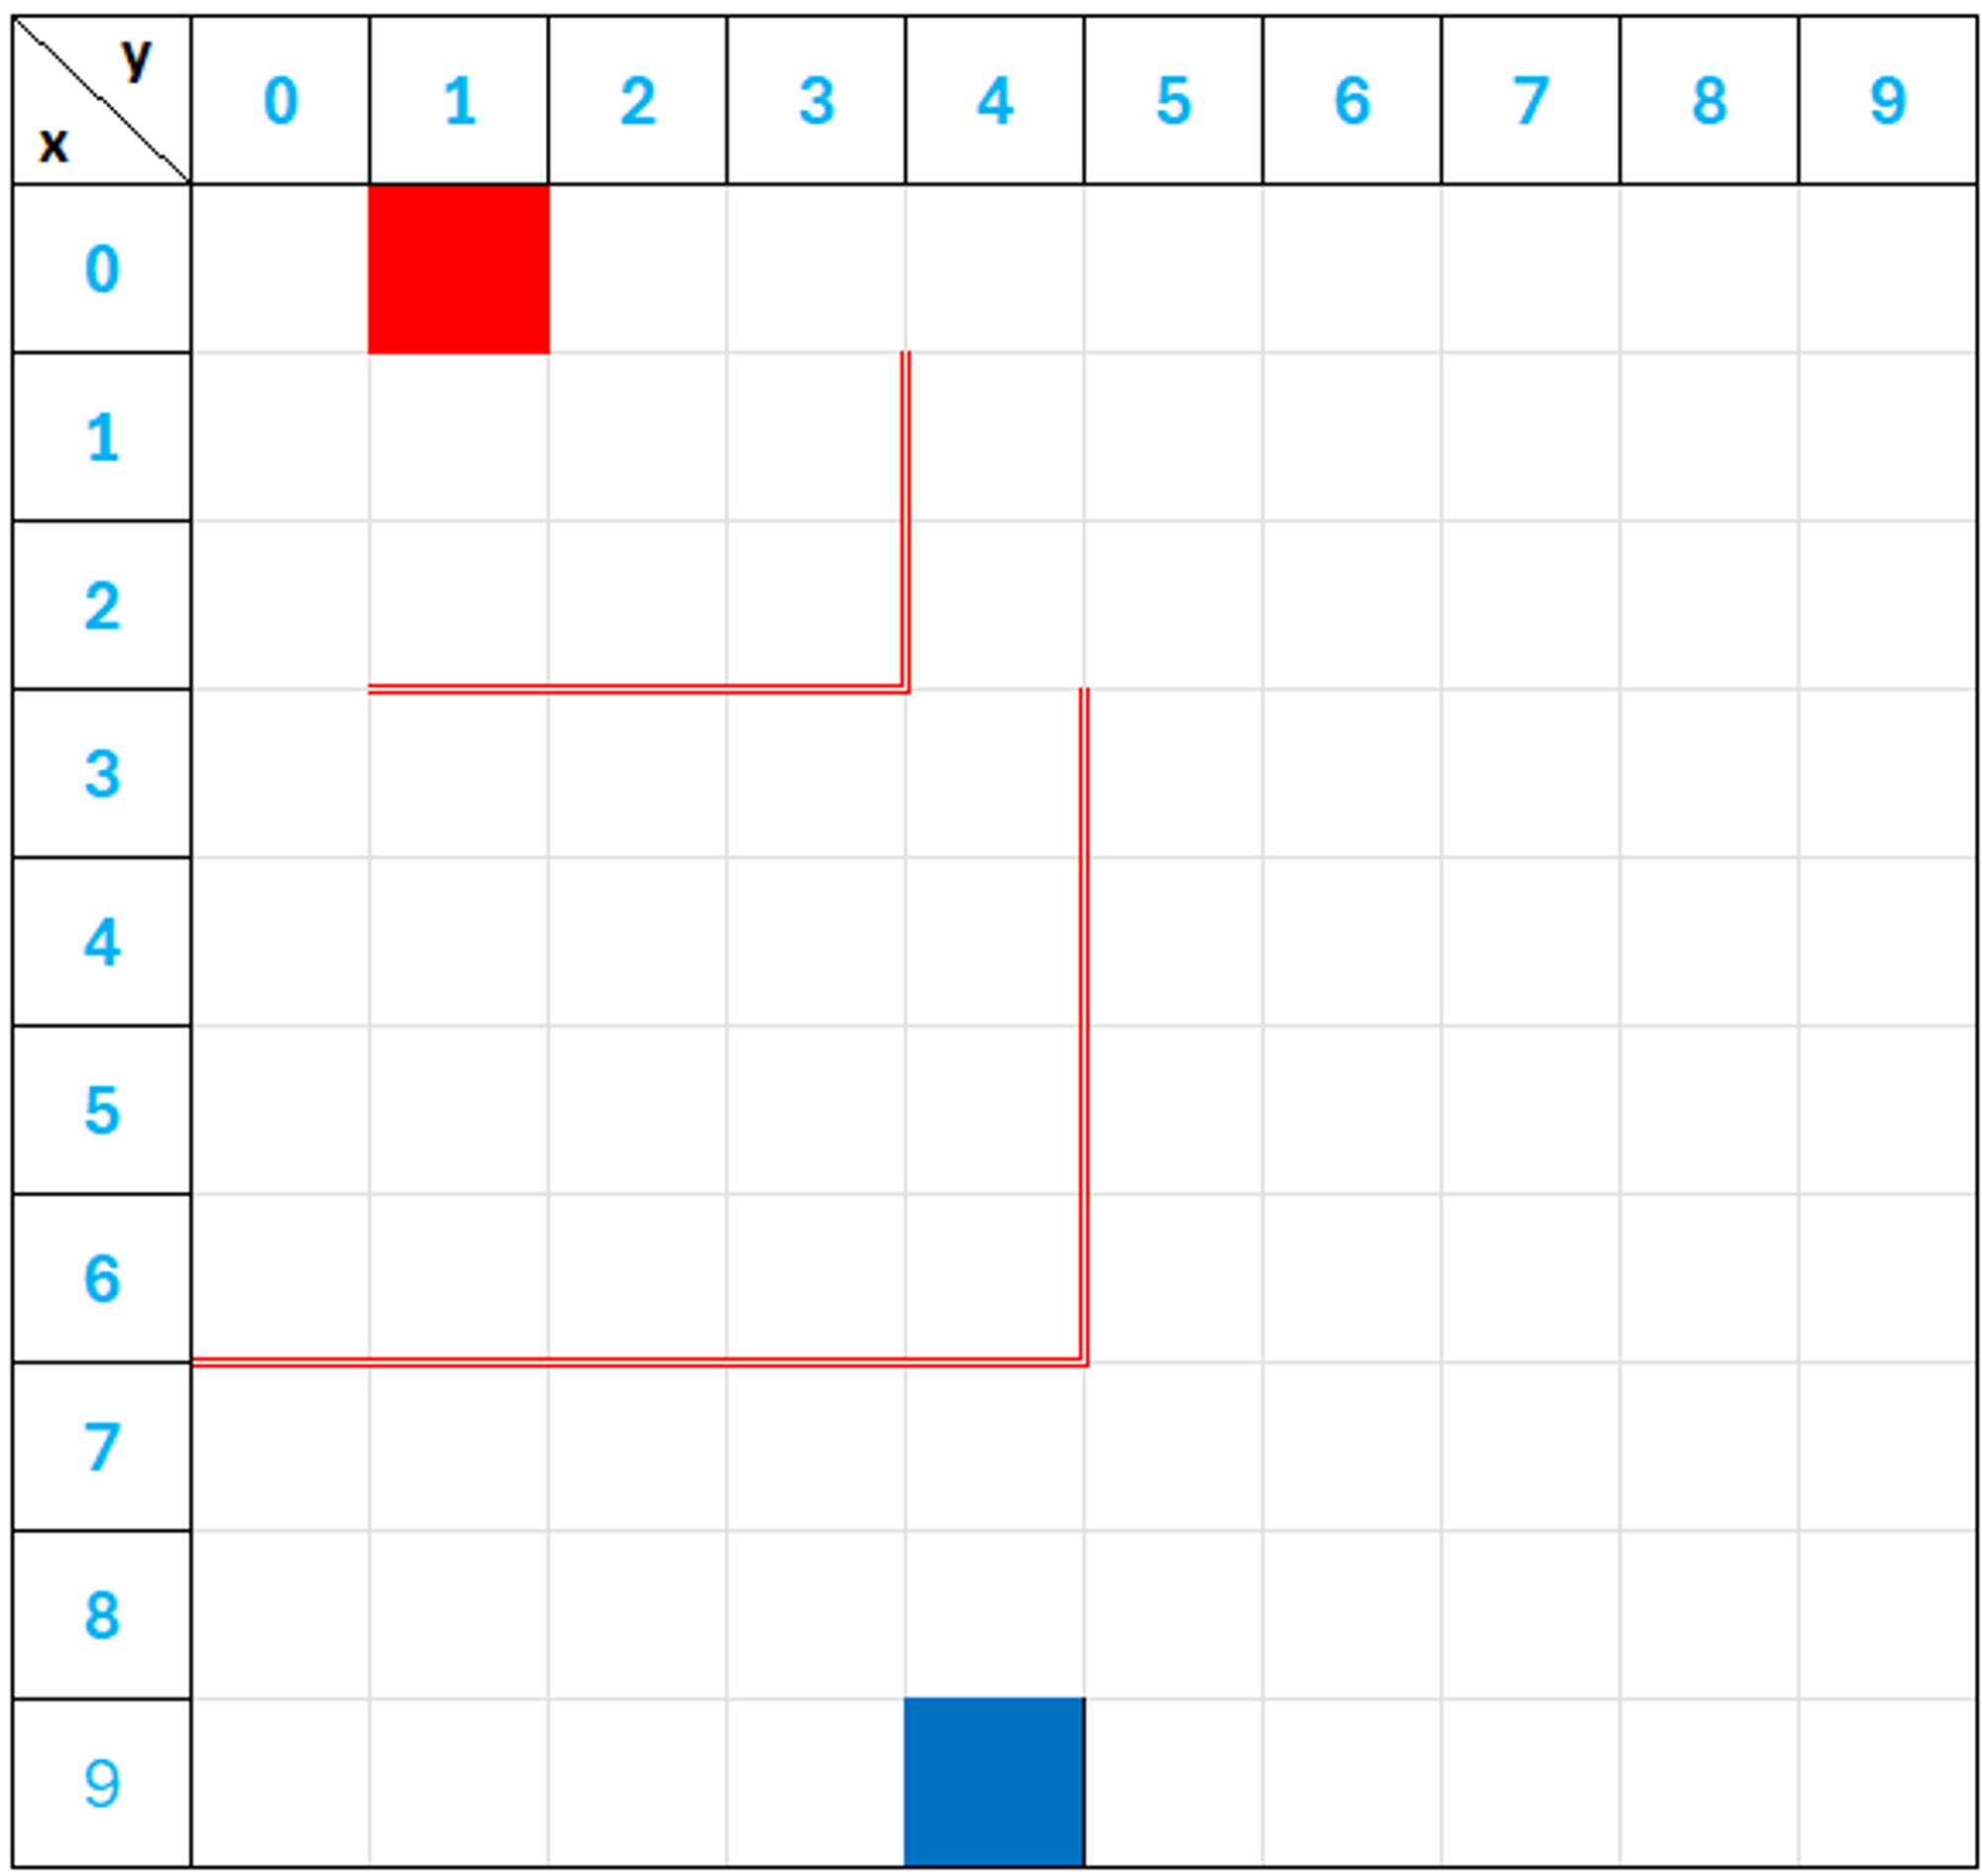
\includegraphics[width=0.5\linewidth]{img/astar_pic1.png}
    \caption{Ma trận giả định với điểm xuất phát, kết thúc và các bức tường}
    \label{fig:astar_pic1}
\end{figure}

\paragraph{}{Sử dụng công thức cho hàm $g(u, v)$ và $h(u, v)$ như đã nói ở trên, ta sẽ có được hai bảng giá trị cho hàm $g$ và $h$ như \hyperref[fig:astar_pic2]{hình 5}.}

\begin{figure}[H]
    \centering
    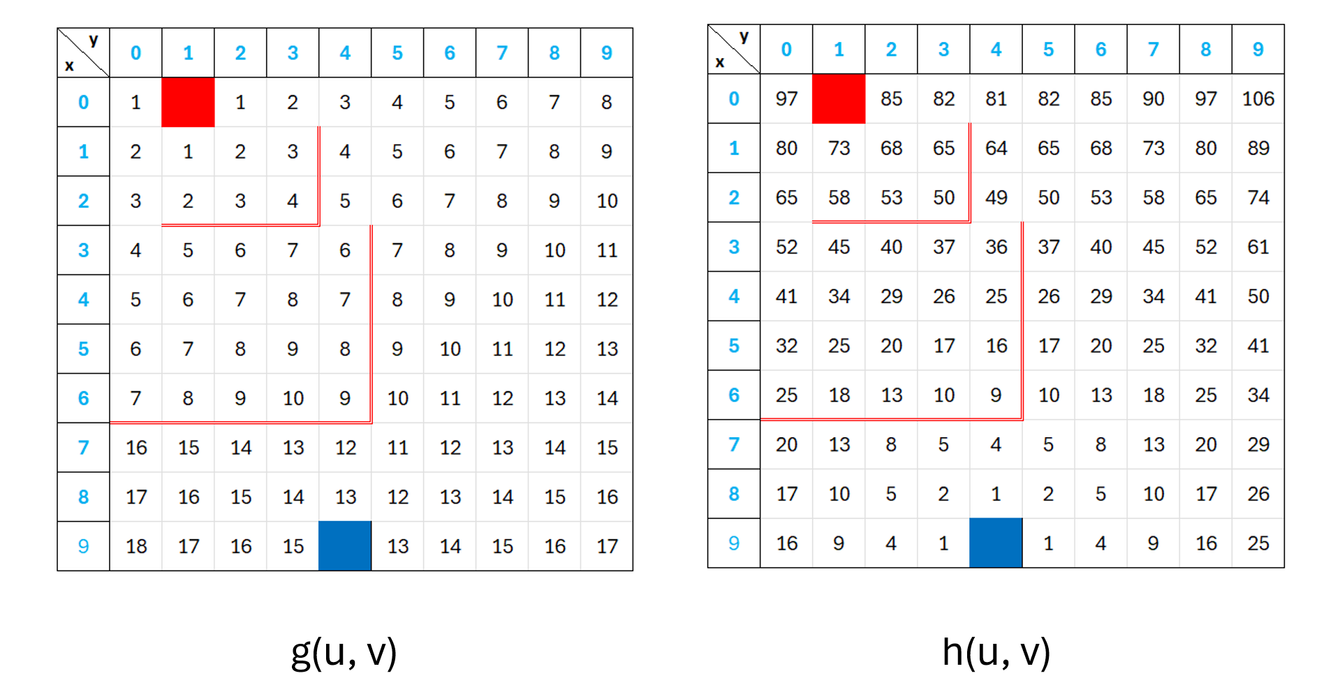
\includegraphics[width=1\linewidth]{img/astar_pic2.png}
    \caption{Bảng giá trị \textit{g} và \textit{h} trong ma trận}
    \label{fig:astar_pic2}
\end{figure}

Vì $f(u, v)$ = $g(u, v)$ + $h(u, v)$ nên ta sẽ có bảng cuối cùng như \hyperref[fig:astar_pic3]{hình 6}:

\begin{figure}[H]
    \centering
    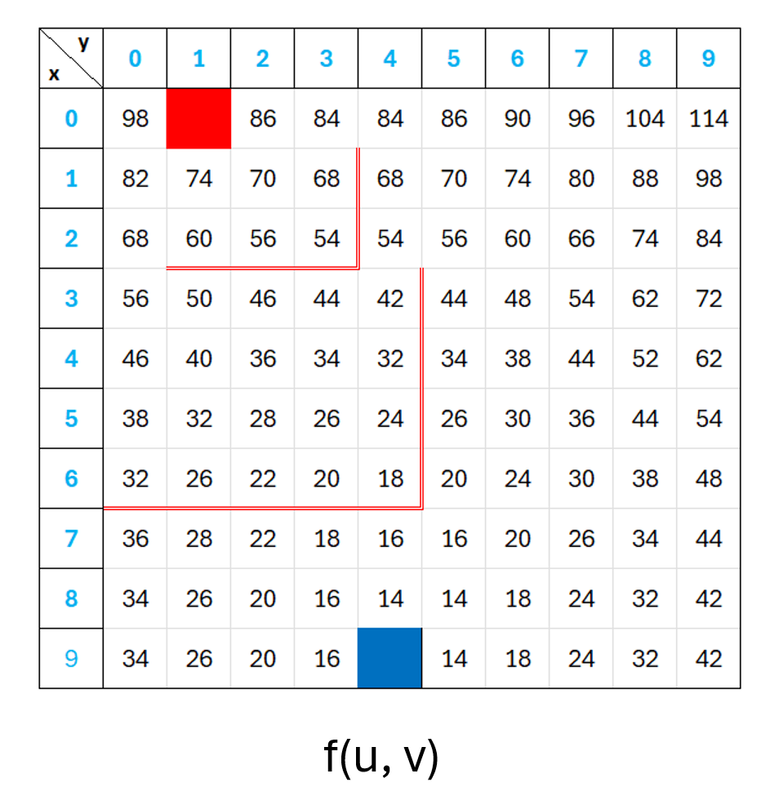
\includegraphics[width=0.5\linewidth]{img/astar_pic3.png}
    \caption{Bảng giá trị hàm \textit{f} trong ma trận}
    \label{fig:astar_pic3}
\end{figure}

Thuật toán khi bắt đầu chạy sẽ xuất phát ở ô màu đỏ là ô $(0, 1)$, duyệt qua các ô chung cạnh xung quanh để tìm một đường đi tới ô kết thúc. Thứ tự duyệt các ô sẽ dựa vào hàm $f(u, v)$ ta vừa tính được, ô có giá trị của hàm $f$ nhỏ hơn sẽ được ưu tiên duyệt trước. Ta có được sơ đồ đường đi của thuật toán như \hyperref[fig:astar_pic4]{hình 7}. Có thể thấy rằng, đường đi được tìm thấy không phải là đường đi ngắn nhất. Đó là bởi vì ta đã bỏ qua tính chất đơn điệu của hàm heuristic như đã nói ở trên.

\begin{figure}[H]
    \centering
    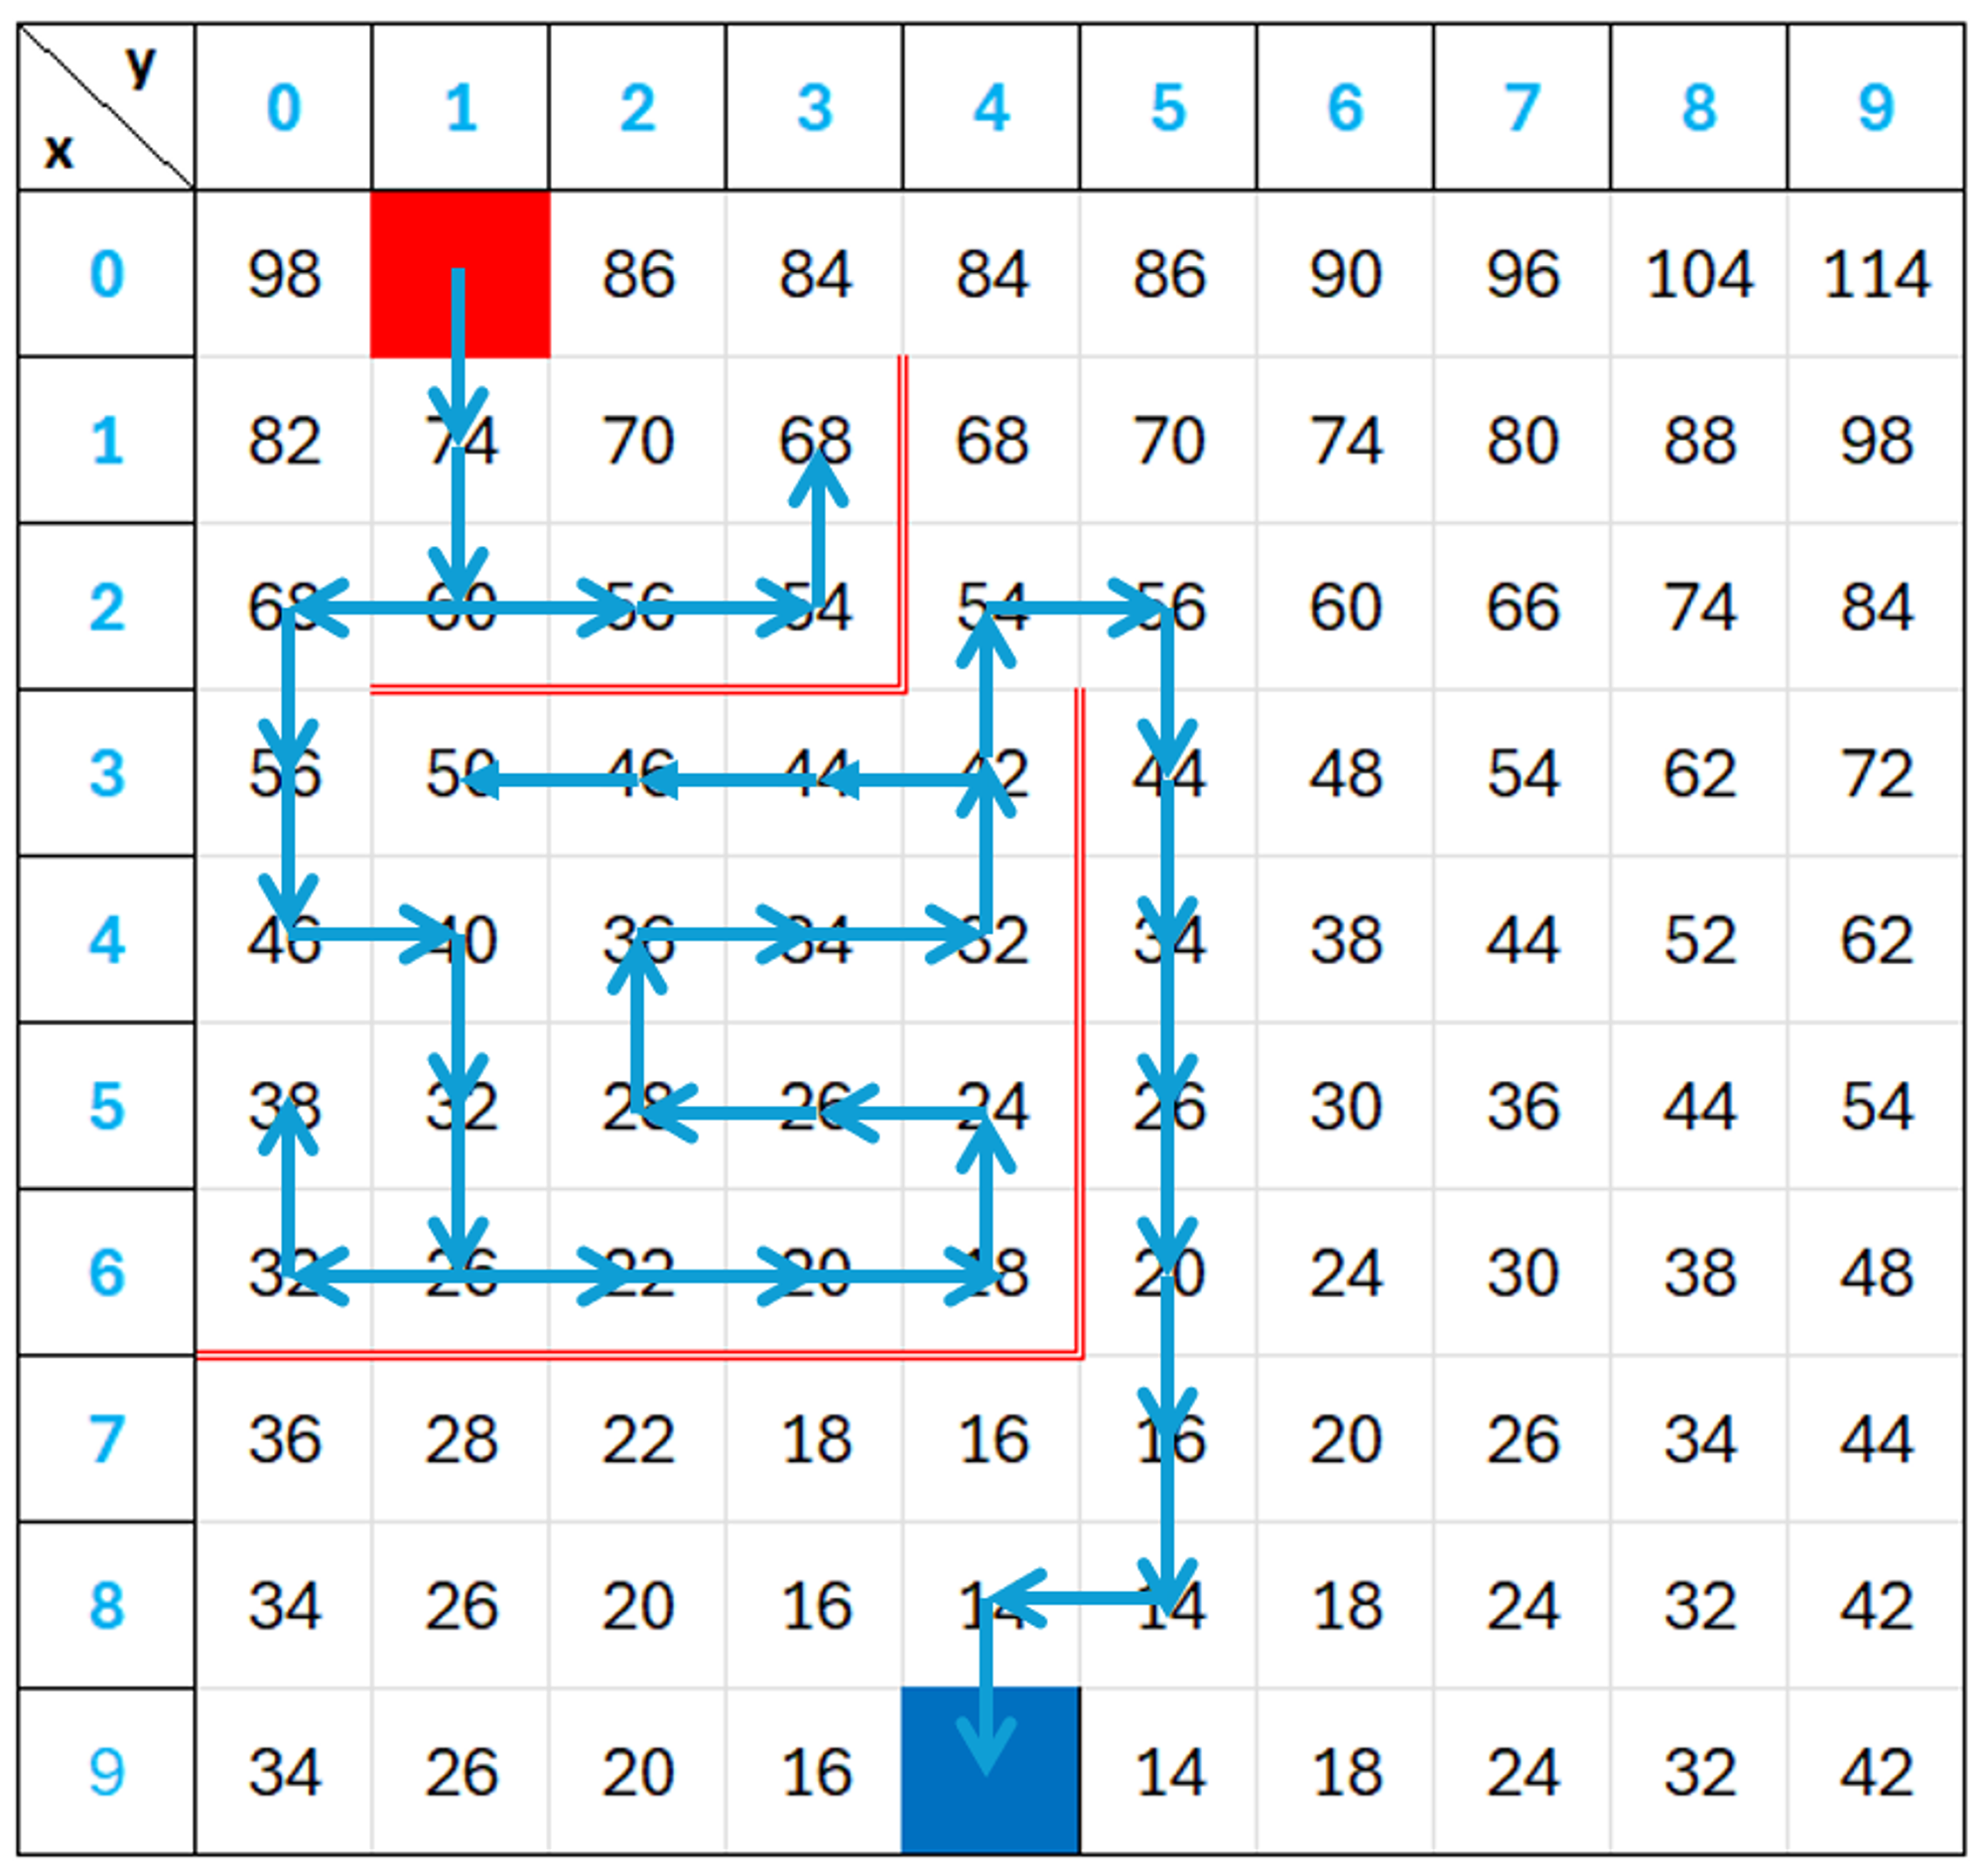
\includegraphics[width=0.5\linewidth]{img/astar_pic4.png}
    \caption{Sơ đồ đường đi thuật toán A*}
    \label{fig:astar_pic4}
\end{figure}

%--------------------------
%      So sanh thuat toan
%--------------------------

\subsection{So sánh thuật toán tìm đường BFS và A*}

\paragraph{Về hiệu suất}

\paragraph{}{Sau 10 lần thử nghiệm và quan sát hai thuật toán A* và BFS với các mê cung kích thước $100 * 100$ khác nhau, chúng tôi có được bảng thống kê thời gian chạy của hai thuật toán này như \hyperref[fig:compare_astar_bfs]{hình 8}:}

\begin{figure}[H]
    \centering
    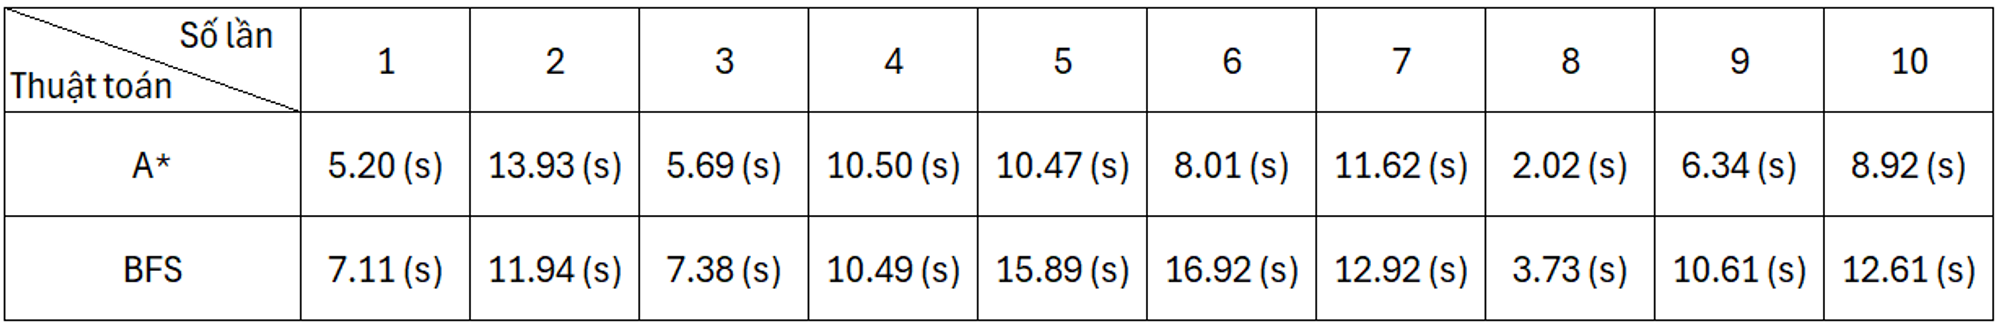
\includegraphics[width=1\linewidth]{img/compare_astar_bfs.png}
    \caption{So sánh thời gian chạy của 2 thuật toán A* và BFS}
    \label{fig:compare_astar_bfs}
\end{figure}

\paragraph{}{Có thể thấy rằng trong đa phần trường hợp, thuật toán A* sẽ có tốc độ nhanh hơn thuật toán BFS. Giải thích cho điều này là vì khác với BFS phải tìm kiếm sang toàn bộ các nút lân cận có cùng độ sâu, thuật toán A* sẽ chỉ ưu tiên tìm kiếm các nút được cho là gần hơn với mục tiêu dựa vào hàm heuristic. Vì vậy, thuật toán A* trong đa phần trường hợp sẽ duyệt qua ít đỉnh hơn so với BFS như \hyperref[fig:compare2_astar_bfs]{hình 9} (ô bắt đầu là ô màu đỏ và ô kết thúc là ô màu xanh). Mặc dù phải duyệt qua ít đỉnh hơn song thuật toán A* vẫn sẽ có trường hợp chạy chậm hơn. Đó là bởi A* sử dụng một hàng đợi ưu tiên (priority queue) có độ phức tạp khi thêm và bớt một phần tử là $O(log(n))$ với $n$ là kích thước của hàng đợi. Trong khi đó, BFS sử dụng một hàng đợi (queue) có độ phức tạp khi thêm và bớt một phần tử là $O(1)$.}

\begin{figure}[H]
    \centering
    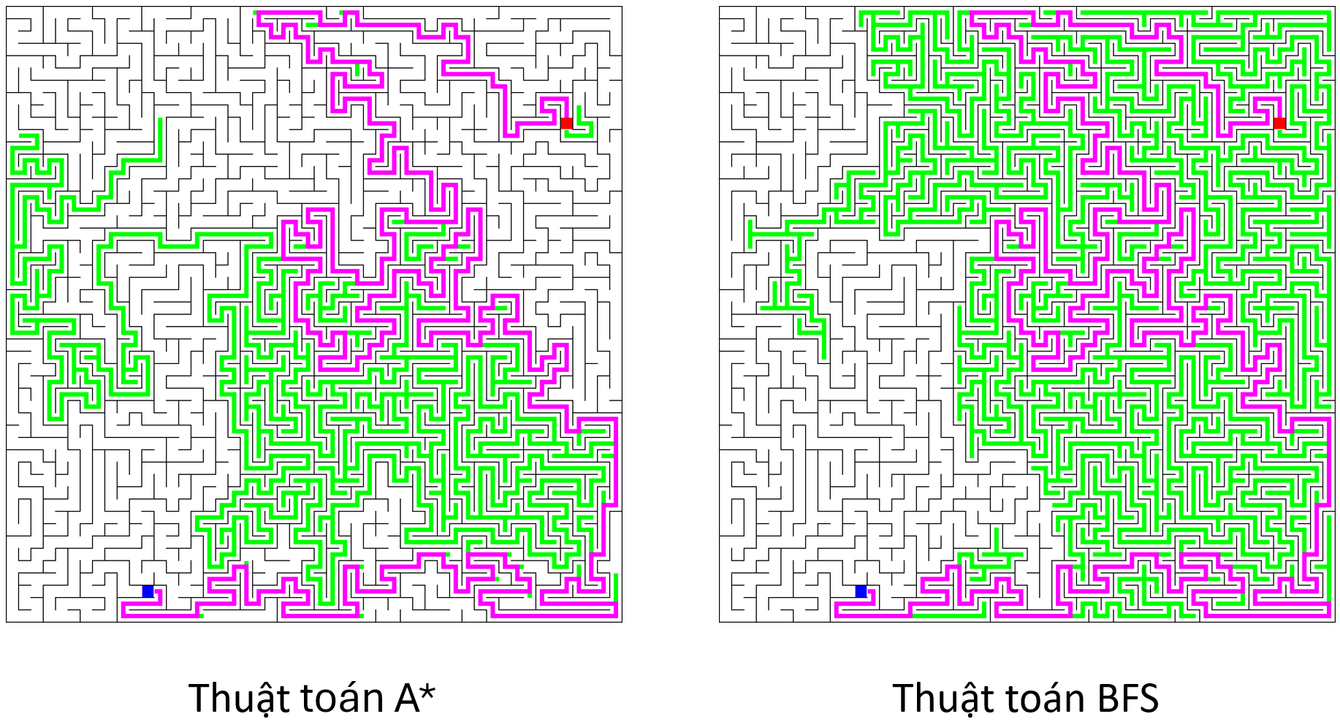
\includegraphics[width=1\linewidth]{img/compare2_astar_bfs.png}
    \caption{Minh hoạ A* và BFS tìm đường trong mê cung}
    \label{fig:compare2_astar_bfs}
\end{figure}

\paragraph{Về bộ nhớ}
\paragraph{}{Cả BFS và A* đều có độ phức tạp về không gian trong trường hợp tệ nhất là $O(|V|)$ với $|V|$ là số nút trong đồ thị. Tùy vào trường hợp đồ thị phức tạp hay không, bộ nhớ sử dụng của BFS sẽ phụ thuộc vào số nút được lưu giữ vào hàng đợi (queue). Còn đối với thuật toán A* sẽ là phụ thuộc vào hàm heuristic và số nút được đưa vào hàng đợi ưu tiên (priority queue).}


\subsection{Hệ thống gợi ý đường đi}

\paragraph{}{Để tạo hệ thống gợi ý, ban đầu sau khi sinh ra một mê cung, chúng tôi đồng thời sử dụng thuật toán BFS để xây dựng một đồ thị mới, bắt đầu duyệt từ ô kết thúc và đi tới tất cả các ô khác trong mê cung. Lúc này, đồ thị nhận được là một cây có nút gốc tương ứng với ô kết thúc của mê cung. Và vì đồ thị là một cây nên tại một nút $(x, y)$ bất kỳ, ta biết rằng nút này có duy nhất một nút cha $(u, v)$. Hướng đi từ  ô$(x, y)$ tới ô $(u, v)$ cũng là hướng đi hướng tới ô kết thúc. }

\begin{figure}[H]
    \centering
    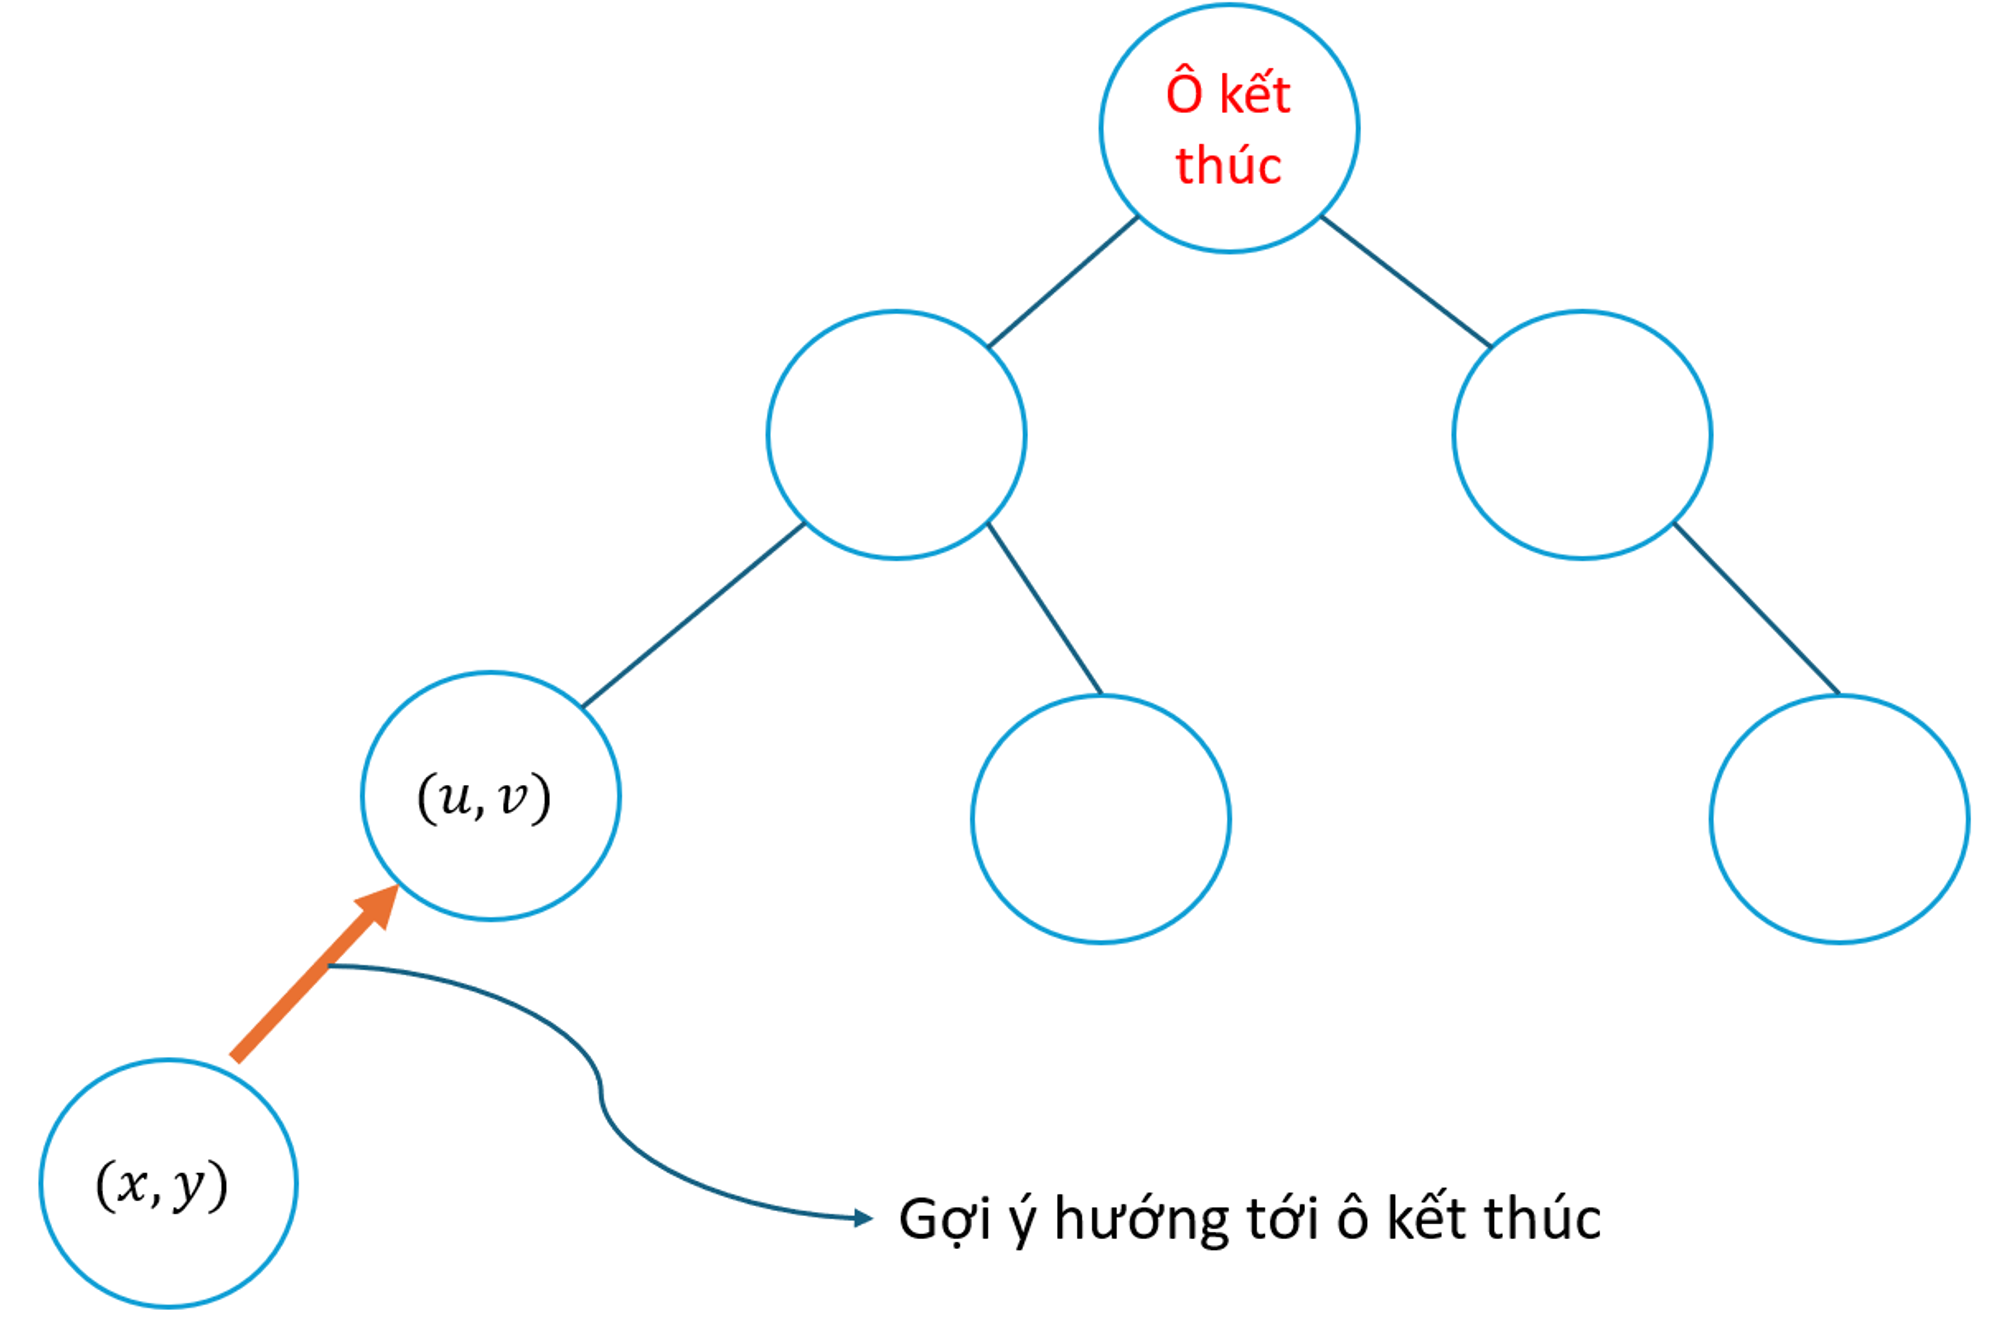
\includegraphics[width=0.7\linewidth]{img/hint_line_1.png}
    \caption{Sơ đồ cây gợi ý}
    \label{fig:hint_line_1}
\end{figure}

\paragraph{}{Sau khi người chơi ấn nút gợi ý, hệ thống sẽ tự động đưa người chơi đi theo con đường duy nhất hướng tới ô kết thúc cho đến khi gặp một ngã ba hoặc ngã tư. Lúc này, người chơi sẽ có thể tiếp tục tự mình chơi tiếp hoặc có thể ấn nút gợi ý một lần nữa.}

\begin{figure}[H]
    \centering
    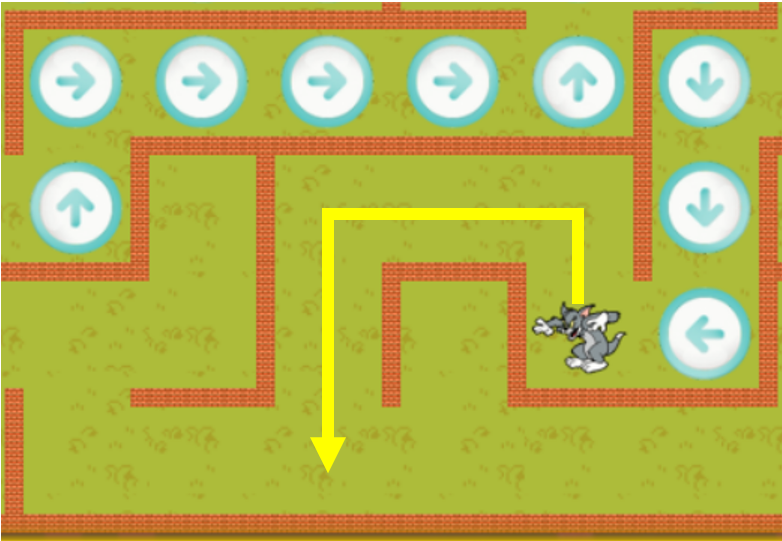
\includegraphics[width=0.7\linewidth]{img/hint_line_2.png}
    \caption{Hệ thống sẽ dẫn người chơi đi theo đường màu vàng và dừng ở ngã ba tại đầu mũi tên.}
    \label{fig:hint_line_2}
\end{figure}
\newpage
\section{Lý thuyết trò chơi: Tối ưu đường đi với năng lượng phát sinh ngẫu nhiên}

\subsection{Bài toán và các yêu cầu}

\paragraph{Bài toán}
\paragraph{}{Bài toán được đặt ra như sau: "Cho trước \textbf{số bước đi tối đa} của Tâm là \textbf{H}, và \textbf{phát sinh ngẫu nhiên} \textbf{K} viên năng lượng trong bản đồ. Tìm đường đi ngắn nhất đến nhà Gia Huy, biết rằng cứ mỗi bước đi sẽ mất 1 năng lượng và ăn được 1 viên năng lượng sẽ có thêm $V_k$ năng lượng với $V_k$ là giá trị phát sinh ngẫu nhiên thuộc \{1, 2, 3, 4, 5\}. Giá trị của \textbf{H} và \textbf{K} cũng sẽ tương ứng với các mức độ trò chơi. Hãy trình bày chi tiết đề xuất của bạn về các giá trị này và lý do."}

\paragraph{Phân tích yêu cầu}
\paragraph{}{Dễ thấy bài toán có 2 yêu cầu chính:}
\begin{enumerate}
    \item Cho trước giá trị của H và K. \textbf{Tìm đường đi ngắn nhất} đến đích.
    \item \textbf{Tìm giá trị} của \textbf{H} và \textbf{K} tương ứng với độ lớn của bản đồ (20x20, 50x50, 100x100).
\end{enumerate}
\paragraph{}{và 2 cách mà viên năng lượng được phát sinh:}
\begin{enumerate}
    \item Tất cả viên năng lượng $V_k$ được phát sinh giá trị \textbf{trước khi bắt đầu trò chơi}.
    \item Giá trị viên năng lượng $V_k$ được phát sinh \textbf{khi chạm đến}.
\end{enumerate}

\subsection{Bài toán tìm đường đi ngắn nhất khi $V_k$ được phát sinh khi chạm đến}

\paragraph{Đặt tên các giá trị}
\paragraph{}{Với mỗi ô trong mê cung, ta đều có thể tìm được đường đi ngắn nhất đến đích. Gọi số bước của đường đi này là $S$. Cùng với mỗi ô trong mê cung, ta gọi $H_{now}$ là số bước đi còn lại có thể đi.}
\paragraph{}{Gọi $m$ là số ô năng lượng có thể đi tới. Với $m \ge 1$, gọi $P_i$ ($1 \le i \le m$) là số bước để đi đến ô năng lượng có thể đi tới. $P_1$ là số bước đi đến ô năng lượng gần nhất}

\paragraph{Hướng giải quyết}
\paragraph{}{Trong trường hợp $H_{now}\ge S$ tại ô bất kì, bài toán ngay lập tức được giải.}

\paragraph{}{Ta dễ thấy khi $H_{now} < S$, ta phải tìm cách để đưa $H_{now}\ge S$, điều này chỉ có thể thực hiện khi ta nhận được năng lượng $V_k$. Do đó, tại các ô năng lượng và ô bắt đầu mới tồn tại khả năng cho $H_{now}\ge S$}. Suy ra, ta phải đi đến: hoặc là đích đến (nếu $H_{now}\ge S$), hoặc là một trong các ô năng lượng có thể di chuyển tới được.

\paragraph{}{Từ vị trí đang đứng, nếu $H_{now} < P_1$ hay $m = 0$ (điều kiện $H_{now} < S$), ta không tìm được đường đi đến đích, bài toán kết thúc.} Ngược lại, nếu $H_{now} \ge P_1$ hay $m \ge 1$, ta sẽ \textbf{chọn ô năng lượng} \texttt{good} ($1 \le good \le m$) để di chuyển tới, với $\left| (H_{now}-P_{good} + 1)-S_{good} \right|$ \textbf{đạt giá trị nhỏ nhất} (tức là càng tiến sát tới mục tiêu tìm được đường đi: $H_{now} \ge S$)

\subsection{Bài toán tìm đường đi ngắn nhất khi $V_k$ được phát sinh trước khi bắt đầu trò chơi}



\subsection{Đề xuất các giá trị H và K}

\paragraph{Đề xuất các giá trị H và K}
\paragraph{}{Chúng tôi đề xuất $H = 1,5 \times S$, $K = 0,2 \times level^{2}$, với $S$ là số bước đi ít nhất để đến đích và $level \in \{20, 50, 100\}$ tương ứng với các mức độ của trò chơi.}
\paragraph{}{\textbf{Lý do}: Người chơi thông thường sẽ không tìm được đường đi tốt nhất để đi trong mê cung. Vì vậy, đường đi thường lớn hơn giá trị S, chúng tôi chọn $1,5 \times S$ và thêm $2 
\times level^{2}$ viên năng lượng - mật độ phân bố phù hợp với mê cung.}
\newpage
\section{Hướng dẫn cài đặt, minh hoạ trò chơi}

\subsection{Hướng dẫn cài đặt}

\paragraph{Cài đặt Python và các thư viện}
\paragraph{}{Để trò chơi hoạt động, đầu tiên cần cài đặt Python và các thư viện phụ trợ}
\begin{itemize}
    \item python: phiên bản $3.11.9$
    \item pygame: phiên bản $2.5.2$
    \item pygame-menu: phiên bản $4.4.3$
\end{itemize}

\paragraph{}{Mở Command Prompt và chạy các lệnh:}
\begin{lstlisting}[language=tex]
pip install python==3.11.9
pip install pygame==2.5.2
pip install pygame-menu==4.4.3
\end{lstlisting}

\paragraph{Cài đặt game}
\paragraph{}{Tải file game từ Github: \href{https://github.com/htrung1105/MazeGame}{https://github.com/htrung1105/MazeGame}}.

\paragraph{Bắt đầu game}
\paragraph{}{Vào thư mục game đã tải, chạy file \texttt{main.py}}

\subsection{Minh hoạ trò chơi}

\paragraph{Demo}
\paragraph{}{Video demo trò chơi:}
\paragraph{}{\href{https://www.youtube.com/playlist?list=PLrrNR4O04Hcso0\_6GI8eDOB5dsBtBEIS3}{https://www.youtube.com/playlist?list=PLrrNR4O04Hcso0\_6GI8eDOB5dsBtBEIS3} }

%\paragraph{Hình ảnh minh hoạ}
%\paragraph{}{Sau đây là một vài hình ảnh trong game:}



\cleardoublepage
\phantomsection
\addcontentsline{toc}{section}{Tài liệu tham khảo}
\bibliographystyle{unsrt}
\bibliography{ref/ref}

\end{document}